% Paper 2A, version 18 (4 October 2026)
\documentclass[11pt]{article}
\usepackage[utf8]{inputenc}
\usepackage[T1]{fontenc}
\usepackage{lmodern}
\usepackage{amsmath,amssymb,amsthm}
\usepackage{tikz,tikz-cd}
\usetikzlibrary{arrows.meta,positioning,shapes.geometric}
\usepackage[margin=1in]{geometry}
\usepackage[round,authoryear]{natbib}
\usepackage{booktabs,array,tabularx,placeins,microtype}
\usepackage[hidelinks]{hyperref}
\usepackage{xurl}
\setlength{\emergencystretch}{3em}
\widowpenalty=10000
\clubpenalty=10000
\displaywidowpenalty=10000
\makeatletter
\setlength{\@fptop}{0pt}
\makeatother
\newcolumntype{L}{>{\raggedright\arraybackslash}X}
\newcolumntype{P}[1]{>{\raggedright\arraybackslash}p{#1}}
\theoremstyle{definition}
\newtheorem{definition}{Definition}[section]
\newtheorem{proposition}{Proposition}[section]
\newtheorem{corollary}[proposition]{Corollary}
\newtheorem{lemma}[proposition]{Lemma}
\newtheorem{remark}{Remark}[section]
\newcommand{\code}[1]{\texttt{#1}}

\title{Copied Agreement: Lineage-Grounded Audits of\\ Claim Preservation in Data Migration}
\author{Duston Moore}
\date{Version 18, 4 October 2026}
\begin{document}
\maketitle
\begin{abstract}
Equal outputs before and after a schema migration can reproduce a common error when the target is populated from an inadequate source. This paper gives an audit that separates endpoint determination of a claim, agreement on an exhibited carrier of migrated records, and comparison with a claim-relevant valuation whose production path is recorded. Four conditions on a declared lineage graph expose dependencies relevant to independent corroboration. Disclosure can satisfy a structural condition while leaving its defeater unresolved. One countermodel launders shared derived ancestry; a second passes all four clauses with shared raw input and an independent source that the evaluator ignores. Ground-evaluator justification therefore remains a separate assurance obligation. A retained-value fibre test determines extensional dependence on shared derived ancestry, but supplies no separation witness when the retained tuple is injective. In a synthetic tax-jurisdiction migration with 1,728 seam records, endpoint comparison finds 48 disagreements, while delivery evidence identifies 74 grounding witnesses, including 26 records on which both endpoints agree and both are wrong. These are additional diagnoses even though the old endpoint already fails determination of the jurisdictional claim. A two-record control separately passes determination of the actual claim at both endpoints and endpoint agreement, while failing grounding. For a stably bound fixed ground, two lineage conditions compose across consecutive steps; the other two require stated ancestry conditions or a fresh outer audit. The exact fibre and seam lemmas, lineage decisions, finite retained-value checks, composition conditions and boundary examples are mechanised in Coq. Runtime decision cores are extracted to OCaml; independent reference tests check their handwritten wrappers. Positive assurance remains conditional on model relevance, evaluator justification, coverage, source fidelity, resolved defeaters and custody.
\end{abstract}

\section{The claim made by a migration}\label{ex:sec:intro}
A schema migration often offers evidence of success in the form of equal outputs. The old and new implementations compute the same status on tested records, the dual write completes, and updating either side appears to commute with translation. The equality is real. Its relevance depends on the proposition the status is meant to establish and on the production of the two compared values. If the new field was populated from an inadequate old field, agreement can be a record of copying.

The audit developed here asks whether the inputs determine the promised claim, whether its old and new evaluations agree on the migrated records, and whether that agreement is supported by an independently produced ground. A positive answer to one question supplies no answer to the next. Section~\ref{ex:sec:case} shows the three questions coming apart on one synthetic migration.

\paragraph{Running example: a copied tax determination.} A synthetic retailer replaces a postal-zone field with a municipality field. Its old tax pipeline observes the zone, goods class, period, and charged rate. The new pipeline stores a municipality and applies a municipality-keyed table. Live rows are geocoded from the delivery address, but historical rows are backfilled by assigning the primary municipality of the old zone. Four zones also serve a secondary municipality. The concrete row
\[
(2,5,\mathit{general},\mathit{before},60)
\]
is the recurring counterexample. It records a delivery to municipality~5 in zone~2, but the backfill assigns zone~2's primary municipality. On this row the old flag and the new copied flag both report the same result. A separately recorded delivery scan identifies municipality~5 and shows that the common result rests on the wrong jurisdiction. The paper will reuse this row to distinguish four questions: whether the old observation can determine the jurisdictional claim, whether old and new coordinates agree, whether a separately produced seam valuation agrees with them, and whether the production path of that valuation is independent of both coordinates. Section~\ref{ex:sec:case} gives the complete executable case and its counts.

The distinction has a philosophical provenance, but none of the formal results depends on it.\footnote{A Whiteheadian motivation is that symbolic systems can remain internally orderly after their relation to the process has become defective, and that a settled record is not identical with the process from which it was produced \citep{whitehead1927symbolism,whitehead1929}. The engineering development replaces that motivation with tests stated in factorisation, provenance, lineage, coverage, and custody.}

\paragraph{Audience and practical rule.} The primary audience is data engineers, auditors, and formal-methods researchers responsible for claims that must survive migration rather than merely for records that must be copied. The governing rule is: do not treat endpoint equality as evidence that a claim survived a migration unless the claim is determined by the relevant observation surfaces, the migration seam is exhibited with declared coverage, and the seam valuation is grounded by a production path that neither descends from either coordinate nor silently reuses their shared ancestry. The paper develops each obligation separately so that a failed claim has a location and a repair.

\paragraph{Contributions.} The contributions are:
\begin{itemize}
\item A decomposition of claim preservation through migration into endpoint determination, seam coherence on an exhibited carrier, and grounded coherence against a lineage-qualified valuation, with structural passing separated from certificate issuance (Sections~\ref{ex:sec:seams} and~\ref{ex:sec:evolution}).
\item Lineage conditions (L1)--(L4) that make production-path dependencies of the proposed ground auditable on a declared provenance graph, including countermodels for shared derived ancestry and an ignored independent raw source, and a fibre test for extensional dependence on retained shared-ancestry values on a finite carrier, with its injective-carrier limit (Section~\ref{ex:sec:laundering}).
\item An exact composition analysis for a fixed ground: (L1) and (L4) compose across consecutive seams, while (L2) and (L3) carry over exactly under stated ancestry conditions, so a composite certificate needs either those conditions or a fresh outer audit (Section~\ref{ex:sec:lineage-composition}).
\item A Coq development of the exact core, extracted runtime seam, lineage and retained-value decision cores, and a finite tax-jurisdiction audit in which the ground exposes 26 copied-agreement errors missed by endpoint comparison, with observational, stale-table and backfill failures separated (Section~\ref{ex:sec:case}).
\end{itemize}
The fibre criterion is a standard factorisation result and is stated as the observational baseline, not as a contribution.

\paragraph{Relation to the calculus companion.} \emph{Grounded Transport} develops a proof-relevant rewriting calculus for the same setting: witness identity and composition, algebraic laws, erasure, scopes, contexts, and evidence-bearing assessment \citep{moore2026transport}. This paper develops the migration diagnosis, the case study, and the lineage conditions and their composition. Bounded-error extensions require a separately specified metric treatment; no metric supplement is included in the present artefact. A composition of already certified calculus witnesses does not by itself establish that an unexamined outer coordinate pair satisfies the migration lineage conditions: the calculus carries supplied evidence, while this paper asks which evidence the migration must supply. The companion's pinned implementation checks (L1)--(L3), not (L4), and mechanises analogous fixed-ground composition results with different countermodels (Section~\ref{ex:sec:lineage-composition}). Each paper states the shared definitions it needs; their contributions and verification evidence are separate.

\paragraph{Scope.}
The audit concerns exact claim preservation on declared models and carriers. It supplies neither general database semantics nor a complete SQL-equivalence procedure, statistical calibration theorem or proof of exhaustive process capture. The current artefact mechanises the lineage, finite retained-value and composition decisions and extracts their runtime cores; string encoding, retention validation and presentation remain tested wrappers. The original tax/static factor checker remains handwritten. Ground-evaluator justification, clearance and certificate issuance are assurance obligations. Appendix~\ref{ex:app:mechanisation} maps the current claims to their proofs and runtime boundary; Appendix~\ref{ex:app:history} retains the detailed implementation history. No metric supplement or verified bounded-error result is included in this artefact.

\paragraph{Organisation.} Section~\ref{ex:sec:related} relates the audit to migration testing, differential testing, truth discovery, and provenance. Section~\ref{ex:sec:static} states the static baseline and the vocabulary of application warrant. Section~\ref{ex:sec:seams} introduces the migration seam, grounding, and the lineage conditions, and Section~\ref{ex:sec:evolution} treats evolution and composition. Section~\ref{ex:sec:observational} describes how endpoint evidence enters the audit and gives the finite reference procedure. Section~\ref{ex:sec:case} works the tax case, Section~\ref{ex:sec:practice} gives the practical procedure, and Sections~\ref{ex:sec:limitations} and~\ref{ex:sec:conclusion} state limitations and conclude.

\begin{table}[htbp]
\centering
\small
\caption{Core notation.}
\label{ex:tab:notation}
\begin{tabularx}{\textwidth}{@{}P{2.8cm}L@{}}
\toprule
Symbol & Meaning \\
\midrule
$S$, $S_t$ & Declared state model, or the state model at stage $t$ \\
$M:S\to O$ & Observation map from states to the declared observation surface \\
$\Phi:S\to 2$ & Exact predicate whose determination is claimed \\
$\chi$; $\chi_t$ & Declared claim, and its evaluation on the stage-$t$ state model \\
$A_t,B_t$ & Concurrent old and new coordinate models at window stage $t$ \\
$R_t$ & Migration seam carrier accountable under both coordinate descriptions \\
$p_t,q_t$ & Projections from the seam carrier to old and new coordinate state models \\
$\Phi_{R,t}$ & Claim-relevant valuation evaluated on the seam from process evidence \\
$L$ & Declared finite lineage graph for the coordinate and seam valuations \\
$\operatorname{Raw}(L)$, $\operatorname{Rel}(L)$ & Declared raw lineage nodes, and the subset marked claim-relevant \\
$\operatorname{anc}(x)$ & Strict ancestors of node $x$ in the lineage graph \\
$D$ & Shared non-raw ancestry of the two coordinate determinations \\
$E_g$ & Non-raw ancestry shared by the ground and either coordinate \\
\bottomrule
\end{tabularx}
\end{table}

\section{Background and related work}\label{ex:sec:related}\label{ex:sec:formal-neighbours}

\paragraph{Migration testing and data validation.} Standard migration methodology defines correctness relative to the source. Data validation compares source and target databases, and reconciliation maps source identifiers to target identifiers to establish completeness \citep{matthesschulzhaller2011}. The same literature requires reconciliation code to be written afresh rather than copied from the transformation programs it tests, so that their errors are not repeated. Declarative data-quality checking extends such tests to production pipelines: Deequ, for example, lets engineers state constraints and metrics over large datasets and verifies them incrementally \citep{schelter2018}. These methods test fidelity to a source or to declared constraints. They do not ask whether a value faithfully copied from the source was ever correct for the claim it supports. The lineage conditions of Section~\ref{ex:sec:grounding-seam} extend the independence requirement from the checking code to the evidence against which the migrated claim is checked.

\paragraph{Differential testing and the oracle problem.} Comparing old and new evaluations is a form of differential, or back-to-back, testing: comparable systems are run on the same inputs and their disagreements are investigated \citep{mckeeman1998}. Its known limitation is that two systems sharing a fault agree on it. Deciding whether an agreed output is correct is the test-oracle problem \citep{barr2015}. In these terms, seam coherence (Definition~\ref{ex:def:seamcoherence}) is differential testing on the migrated records, and grounded coherence (Definition~\ref{ex:def:grounded-seam}) is oracle-based testing in which the oracle's independence from the systems under test is itself an audited condition, stated over a provenance graph.

\paragraph{Independence of versions and sources.} Knight and Leveson showed experimentally that independently developed versions of one specification do not fail independently \citep{knightleveson1986}. The same point applies to evidence: two separately maintained instruments can share a blind spot. The conditions here concern production-path independence relevant to corroboration; they do not establish independence of failure. In data integration, truth-discovery methods recognise that copying among sources inflates apparent agreement. Dong, Berti-\'Equille, and Srivastava model copying between sources and infer it from shared values, particularly shared false values, so that copied agreement is discounted when deciding which value is true \citep{dong2009}. That work detects dependence statistically across many sources. The present audit instead requires the dependence structure of one seam valuation to be declared and checks it. The two are complementary: statistical copy detection can challenge a declared graph that claims independence, and a declared graph can explain why agreement observed on a carrier should not be counted as corroboration.

\paragraph{Belief merging and repeated sources.}
In the framework of Konieczny and Pino P\'erez, the source profile
is a multiset, allowing repeated beliefs from distinct sources to
affect merging \citep{konieczny2002merging}. Where reports repeat
a common upstream claim, source multiplicity alone does not establish
independent corroboration. The present audit addresses the declared
production paths relevant to that evidential distinction; it does
not define a new belief-merging operator.

\paragraph{Provenance.} Database provenance distinguishes why an output appears from where its values were copied \citep{buneman2001}, and provenance semirings preserve alternative and joint derivations through relational queries \citep{greenkarvounarakistannen2007}. The W3C PROV data model supplies a standard vocabulary for entities, activities, agents, generation, use, and derivation \citep{w3cprovdm2013}. These supply the graph. Conditions (L1)--(L4) are additional, claim-specific constraints over it (Section~\ref{ex:sec:grounding-seam}).

\paragraph{Online schema change.} Production systems change schemas while serving traffic by passing through intermediate schema states that keep concurrently running servers consistent \citep{rae2013}. Such protocols govern when old and new representations may coexist and how data is backfilled. They make the seam carrier of Section~\ref{ex:sec:migration-seam} concrete, but they do not address whether a backfilled value is true of the occurrence it describes.

\paragraph{Categorical data migration.} Functorial data migration models a schema as a small category, an instance as a set-valued functor, and a schema functor as inducing canonical data-migration functors \citep{spivak2012,spivakwisnesky2012}. The seam used here is a different object. $R_t$ is a carrier of process or record instances accountable under both descriptions, and its projections relate those instances to the two coordinate state models. A categorical migration may implement or justify parts of the projections or an observational translation, but categorical preservation alone does not answer whether the carried value has a claim-relevant ground independent of the source coordinate.

\paragraph{Query and application equivalence.} Database verification supplies stronger proof techniques when the relevant semantics can be expressed symbolically. Cosette combines constraint-based counterexample search with proof-assistant reasoning for SQL query equivalence \citep{chucosette2017}; Q*cert mechanises semantics and correctness properties for query-compilation pipelines in Coq \citep{auerbach2017}; and Mediator uses bisimulation invariants to verify equivalence of database-driven applications across schema changes \citep{wang2018}. These methods can discharge obligations that a finite enumeration cannot. They do not, by themselves, establish the completeness of a seam carrier, the independence of a claimed ground, or the accuracy of the raw process evidence. Conversely, the fibre and grounding criteria do not replace query or program equivalence when those are the claims at issue.

\paragraph{Assurance arguments.} Assurance~2.0 treats assurance as an eliminative argument in which identified defeaters must be answered or left explicitly open \citep{bloomfieldrushby2021,bloomfieldnetkachovarushby2024}. The witnesses defined below fit that structure, and the disclosure conditions (L2) and (L4) record defeaters rather than resolve them.

\paragraph{Formal neighbours of the fibre criterion.} The factorisation test of Section~\ref{ex:sec:test} has established relatives: measurable factorisation in the Doob--Dynkin lemma \citep[Lemma~1.13]{kallenberg2002}, Blackwell's comparison of experiments \citep{blackwell1953}, the data-processing inequality \citep{coverthomas2006}, exactness of the Galois abstraction induced by an observation map \citep{cousot1977}, and noninterference when the state space is a product and the observer sees one component \citep{goguenmeseguer1982}. A companion manuscript develops these relations \citep{moore2026exactness}; none is claimed as a contribution here.

\paragraph{Position.} The requirement that a check be independent of what it checks is old. The contribution here is to state that requirement for the evidence used to corroborate a migrated claim, as conditions on a declared lineage graph that can be checked, composed, and reported with their residual assumptions, and to show on a worked case what they detect that endpoint comparison does not.

\section{Claims, observation surfaces, and application warrant}\label{ex:sec:static}

\subsection{Application warrant and continuing reliance}\label{ex:sec:warrant}

\begin{definition}[Application warrant]\label{ex:def:warrant}
Application warrant is the evidential entitlement to assert a specified claim about a concrete case for a stated use and time, conditional on the adequacy of the artefact's construction and on the continuing operation of practices that preserve its claim-relevant distinctions.
\end{definition}

A passing internal check supplies only part of that entitlement. The state model, observation map, and predicate must fit the claim; the observation must determine it; and the instruments, transformations, and evidence must remain adequate after change. Factorisation establishes the determination condition within the declared model. It does not establish the relevance of that model or the fidelity of the instruments that realise it. The justification for those initial choices is \emph{construction warrant}.

\emph{Warrant Debt} is continued institutional reliance on a claim while a necessary condition of its application warrant remains unmet. A defect found and repaired before reliance is not yet debt. The tax case locates unmet conditions in construction, observation, maintenance, and institutional custody so that each repair has an evidential basis and an owner. The wider account is developed separately \citep{moore2026exactness}; the present audit identifies failures and does not infer continued reliance from a witness alone.

A claim is \emph{affirmed} for a declared scope when its warrant conditions are established, \emph{denied} when evidence refutes it, and \emph{underdetermined} otherwise. A clean search supports affirmation only when it is complete for the asserted scope.

\subsection{Static baseline: observation-relative admissibility}\label{ex:sec:test}

The surface $M$ identifies states with the same observed value. Exact determination of $\Phi$ requires $\Phi$ to respect that identification. The test compares the declared map and predicate; it does not establish that either fits the concrete process $\mathcal{C}$.

\subsubsection{The domain}

The model $S$ already embodies choices about occurrences and relevant differences. Let $\mathcal{C}$ be the concrete process, $\iota$ its modelling as $S$, and $M:S\to O$ the declared observation map:
\[
\mathcal{C} \overset{\iota}{\longrightarrow} S \overset{M}{\longrightarrow} O.
\]
The test below concerns whether the predicate $\Phi:S\to 2$ survives $M$. It does not test the placement of $\iota$ or the accuracy of an implemented observation. Examples of $\Phi$ include tenant isolation and the absence of a forbidden transition.

\paragraph{The concrete process is not an oracle.} The notation $\mathcal{C}$ names the process about which the regime makes its claim; it does not assume unmediated access to ``ground truth''. Every operational check reaches the process through instruments, traces, scans, source records, or other evidence. Those records can themselves be wrong or incomplete. The formal contribution is therefore conditional in two different ways. Factorisation asks whether a declared representation preserves the distinctions required by a declared predicate. Grounded migration asks whether the seam valuation has a claim-relevant production path independent of the two coordinates. Neither establishes the accuracy or completeness of the evidence at the start of that path. Those are construction and institutional obligations, and a positive formal result must retain them as stated assumptions.

\begin{definition}[Observation-relative admissibility]\label{ex:def:admissible}
$\Phi$ is $M$-admissible, written $\operatorname{Admissible}_M(\Phi)$, when $\Phi=\widehat\Phi \circ M$ for some map $\widehat\Phi:O\to 2$.
\end{definition}

\paragraph{Engineering reading.} If two concrete cases look identical on the complete input surface $M$, they must require the same answer to the exact claim $\Phi$. In the running example, the old zone-based surface cannot distinguish an order delivered to zone~2's primary municipality from an otherwise identical order delivered to municipality~5. Since the correct jurisdictional answer differs, the old surface cannot determine that claim exactly.

\paragraph{Why this formalism?} The promised relation is exact recovery of $\Phi$ from the complete declared input $M(s)$. States identified by $M$ must then have the same $\Phi$ value. Factorisation tests that requirement. Predictive accuracy is a different property: a predictor may perform well even though one observation fibre contains states with different target values.

Over arbitrary $S$ and $O$, admissibility asserts existence rather than computability. The finite procedure of Section~\ref{ex:sec:finite-procedure} constructs a factor only with a certified complete enumeration of $S$ and decidable equality on $O$. Exact determination from $M$ entails admissibility; admissibility alone does not warrant application:
\[
\text{warrant for exact $M$-based determination of $\Phi$} \;\Longrightarrow\; \operatorname{Admissible}_M(\Phi).
\]
A calibrated estimate does not promise to determine each individual's $\Phi$ and need not satisfy this condition. A computed score $f(M(s))$ trivially factors through $M$ as a score; that does not establish calibration to an outcome or justify an adverse decision. Those claims require an identified outcome and use, sampling and error evidence, and review after changes in population or features. A fibre witness refutes exact recovery, not probabilistic prediction. If a score is used as an exact individual determination, that stronger claim must satisfy the fibre test.

The following lemma is standard; it is the universal property of the quotient of $S$ by the kernel of $M$, and everything later depends on it.

\begin{lemma}[Fibre criterion]\label{ex:prop:fibre}
$\Phi$ is $M$-admissible if and only if, for all $s_1,s_2 \in S$, $M(s_1)=M(s_2)$ implies $\Phi(s_1)=\Phi(s_2)$.
\end{lemma}

\begin{proof}
If $\Phi=\widehat\Phi \circ M$ and $M(s_1)=M(s_2)$, then $\Phi(s_1)=\widehat\Phi(M(s_1))=\widehat\Phi(M(s_2))=\Phi(s_2)$. Conversely, suppose $\Phi$ is constant on every fibre of $M$. Define $\widehat\Phi(o)=1$ when some $s \in S$ satisfies $M(s)=o$ and $\Phi(s)=1$, and $\widehat\Phi(o)=0$ otherwise. If $\Phi(s)=1$, the defining condition holds at $M(s)$. If $\Phi(s)=0$, fibre constancy excludes any $s'$ with $M(s')=M(s)$ and $\Phi(s')=1$. Hence $\widehat\Phi(M(s))=\Phi(s)$ for every $s$.
\end{proof}

\begin{remark}[Constructive qualification]
The converse is classical: the definition of $\widehat\Phi$ decides an existential. In constructive type theory, fibre constancy does not supply that decision; a complete enumeration, decidable equality, an explicit section, or a classical axiom must be added. The accompanying repository contains the checked constructive version, and Appendix~\ref{ex:app:verification} reports its assumptions. The criterion also holds with any nonempty codomain in place of $2$ in classical set theory, using a chosen representative on each nonempty fibre and a default off the image; the displayed Boolean proof itself uses only the decision of an existential. Section~\ref{ex:sec:debt-extensions} uses this generalisation.
\end{remark}

A witness refutes admissibility. A factorisation proof or complete finite check establishes it within the declared model. An incomplete clean search returns \code{NoWitnessFound}, corresponding to an unresolved observational assessment rather than a positive certificate, in keeping with Dijkstra's observation about testing \citep{dijkstra1970}. No internal result establishes the model's relevance to the concrete process.

\begin{definition}[Observational witness]\label{ex:def:witness}
An observational witness for $(M,\Phi)$ is a pair $s_1,s_2 \in S$ with $M(s_1)=M(s_2)$ and $\Phi(s_1) \neq \Phi(s_2)$.
\end{definition}

\paragraph{Engineering reading.} A witness is a two-row counterexample: the system sees the same declared inputs but the promised exact answer differs. The running case supplies the pair $(2,2,\mathit{general},\mathit{before},60)$ and $(2,5,\mathit{general},\mathit{before},60)$. No downstream function of the old surface alone can recover which municipality received the order.

\begin{proposition}[No recovery by post-processing]\label{ex:prop:norecovery}
Let $f:O\to Y$ be any map. If $M(s_1)=M(s_2)$, then $(f \circ M)(s_1)=(f \circ M)(s_2)$. Hence no procedure whose input is only $M(s)$ recovers a distinction that $M$ identifies.
\end{proposition}

\begin{proof}
Apply $f$ to both sides of $M(s_1)=M(s_2)$.
\end{proof}

\begin{remark}[Randomised post-processing]\label{ex:cor:no-stochastic-recovery}
The same holds for a randomised procedure. If $K:O\to\mathcal{P}(Y)$ assigns to each observation the output distribution of a possibly randomised post-processor, where $\mathcal{P}(Y)$ is the set of probability distributions on $Y$, then $K(M(s_1))=K(M(s_2))$ at any observational witness, so no such procedure distinguishes the two witness states by their output laws.
\end{remark}

Post-processing $M(s)$ cannot recover a distinction already lost by $M$. A classifier may still estimate $\Phi$ using distributional assumptions, but high held-out accuracy is compatible with a fibre witness. The tax case of Section~\ref{ex:sec:case} supplies one: two orders from the same postal zone have different correct municipalities.

One refinement is always formally available but supplies no operational repair without an additional instrument: the pairing $\langle M,\Phi \rangle$ makes $\Phi$ admissible trivially, because it presupposes an instrument that observes $\Phi$. A refinement repairs observational debt only if the added component is something the regime can observe. Whether it can is a question of construction warrant, not of factorisation.

Write $\ker M$ for the equivalence relation $\{(s_1,s_2)\in S\times S\mid M(s_1)=M(s_2)\}$. Lemma~\ref{ex:prop:fibre} says that $\Phi$ is $M$-admissible if and only if $\ker M \subseteq \ker \Phi$, which locates the minimal formal repair.

\begin{proposition}[Coarsest admissible refinement]\label{ex:prop:shell}
For any map $M':S\to O'$, $\Phi$ is $M'$-admissible if and only if $\ker M' \subseteq \ker \Phi$. In particular, among maps whose kernels refine $\ker M$, the coarsest kernel on which $\Phi$ is admissible is $\ker \langle M,\Phi \rangle=\ker M \cap \ker \Phi$.
\end{proposition}

\begin{proof}
The first claim is Lemma~\ref{ex:prop:fibre}. If $\ker M' \subseteq \ker M$, then $\ker M' \subseteq \ker \Phi$ holds if and only if $\ker M' \subseteq \ker M \cap \ker \Phi$, and $\ker M \cap \ker \Phi=\ker \langle M,\Phi \rangle$ is itself admissible.
\end{proof}

For abstraction domains induced by partitions, Proposition~\ref{ex:prop:shell} is a one-predicate case of complete-shell refinement \citep{giacobazziranzatoscozzari2000,ranzatotapparo2004}: adding the truth set of $\Phi$ splits exactly the mixed blocks of $M$. It identifies the minimal formal refinement, not an observation that can be built. The surface $\langle M,\Phi \rangle$ presupposes an instrument that observes $\Phi$, and a regime can refine only by maps it can realise, so the minimal realisable refinement may be strictly finer than $\ker M\cap\ker\Phi$. Which refinement a regime can instrument is a question of construction warrant.


\section{Seams and grounded coherence}\label{ex:sec:seams}\label{ch:change}

The dynamic analysis has four steps. It first asks whether an earlier certificate remains applicable after change. It then exhibits the migration seam and tests extensional seam coherence. Third, it strengthens that test with coherence against a lineage-qualified valuation. Finally, Section~\ref{ex:sec:evolution} checks whether the seam and its coordinate descriptions evolve functorially across the declared interval and how seams compose. These obligations are cumulative: success at a later step does not repair failure at an earlier one. Throughout, continuity means preserving the distinctions on which a claim depends, not merely retaining a value or copying a record.

\subsection{Dynamic admissibility}\label{ex:sec:dynamic}

\begin{definition}[Dynamic observation regime]
A dynamic observation regime is a family $\{M_t:S_t\to O_t\}_{t \in T}$, indexed by a linearly ordered set of stages $T$ in which each non-final stage $t$ has an immediate successor $t+1$, together with, for each such consecutive pair, transition data $\Gamma_t$ relating $(S_t,M_t,\Phi_t)$ to $(S_{t+1},M_{t+1},\Phi_{t+1})$: a span relating the two state models (defined below), the change of observation surface, and the change, if any, of the predicate.
\end{definition}

\paragraph{Engineering reading.} Treat each deployment stage as a versioned observation contract. The transition record must say what changed in the state model, which fields or instruments changed, and whether the claim itself changed. A schema version number alone is not enough.

The transition data are a record, not a morphism in a category of regimes; no such category is defined or needed here. The only mathematical structure the article imposes on them is the span of Section~\ref{ex:sec:migration-seam} and the evolution maps of Section~\ref{ex:sec:functorial-transport}. The stages need not describe a single monolithic cut-over. Rolling deployments, dual-write periods, and distributed services can be represented by successive stages and overlapping seam carriers, provided the claim-bearing records, their coverage, and their responsible custodians are declared. The framework does not require synchronous consistency or one central database; it requires an auditable relation for the claim being transported.

\begin{definition}[Warrant Debt after a transition]\label{ex:def:dynamic-debt}
An institution incurs Warrant Debt when it continues to rely on the assertion of $\Phi_{t+1}$ for a specified use while an unmet condition of application warrant persists, for example when it carries an earlier certificate across a change that removed a distinction required by $\Phi_{t+1}$. A defect detected before such reliance calls for repair or withholding the assertion; it does not by itself incur debt.
\end{definition}

\paragraph{Engineering reading.} A detected migration defect is a repair item. It becomes Warrant Debt when the organisation keeps using the affected determination while the required evidence or repair remains open.

\begin{corollary}[Dynamic fibre criterion, fixed state model]\label{ex:cor:dynfibre}
Let $S$ be common to stages $t$ and $t+1$, with maps $M_t:S\to O_t$ and $M_{t+1}:S\to O_{t+1}$, and let $\Phi_{t+1}:S\to 2$. A certificate for $\Phi_{t+1}$ that uses only $M_t$ is admissible if and only if $\Phi_{t+1}$ is constant on every fibre of $M_t$.
\end{corollary}

\begin{proof}
Lemma~\ref{ex:prop:fibre} with $\Phi_{t+1}$ for $\Phi$ and $M_t$ for $M$.
\end{proof}

\begin{proposition}[Certificate expiry]\label{ex:prop:certificate-expiry}
An admissibility certificate is regime-indexed: in general,
\[
\operatorname{Admissible}_{M_t}(\Phi_t)
\not\Longrightarrow
\operatorname{Admissible}_{M_{t+1}}(\Phi_{t+1}).
\]
The non-implication already occurs (a) when the later surface is an information-losing coarsening and the predicate is unchanged, and (b) when the surface is unchanged and the predicate is redefined.
\end{proposition}

\begin{proof}
For (a), let $S=2$, $M_t=\operatorname{id}_2$, $M_{t+1}$ be constant, and $\Phi_t=\Phi_{t+1}=\operatorname{id}_2$. The stage-$t$ predicate is admissible, while $0$ and $1$ form an observational witness at $t+1$. For (b), let $S=2$ again, let both surfaces be the constant map $S\to\{*\}$, let $\Phi_t$ be constant, and let $\Phi_{t+1}=\operatorname{id}_2$. Again the earlier predicate is admissible and the later one is not.
\end{proof}

Not every change destroys admissibility: an unchanged $\Phi$ remains admissible if $M_{t+1}$ distinguishes at least what $M_t$ did. The actual transition, however, must be checked before the earlier certificate is used. Continued reliance without that review may incur maintenance Warrant Debt (Section~\ref{ex:sec:warrant}).

\subsection{The migration seam}\label{ex:sec:migration-seam}

In the running tax example, a seam element is one order represented under both schemas during the migration window. Live dual-writes and historical backfill rows are different seam origins because they have different production paths. The seam therefore records not only which old and new rows correspond, but how the corresponding pair entered the migration.

When a system is re-architected, old and new states are not the same objects, and relating $S_t$ to $S_{t+1}$ requires a span
\[
S_t \xleftarrow{\;p_t\;} R_t \xrightarrow{\;q_t\;} S_{t+1},
\]
where $R_t$ records the pieces of process accountable to both an old state and a new one, such as a request in flight during a deployment or a record migrated and not yet re-indexed. In an online schema migration from a free-text address field to a structured one, a request that dual-writes during the migration window is an element of $R_t$, read under the old shape by $p_t$ and committed under the new shape by $q_t$. A runbook that logs its dual-written requests exhibits $R_t$; one that does not leaves any claim that certificates survived the migration without the object over which the claim could be checked. Section~\ref{ex:sec:case} works this migration through with a tax-jurisdiction claim.

This set-level span is the audit object; Section~\ref{ex:sec:related} contrasts it with categorical data migration.

\begin{definition}[Exhibited seam]\label{ex:def:exhibited-seam}
A migration seam for a claim consists of (a) a mathematical span
\[
S_t\xleftarrow{p_t}R_t\xrightarrow{q_t}S_{t+1},
\]
and (b) an assurance record $\rho_t$. It is \emph{exhibited} when the record supplies (i) stable identifiers for the relevant carrier elements; (ii) provenance linking each element through $p_t$ and $q_t$ to one declared process; (iii) evidence sufficient to evaluate the claim-relevant seam valuation; (iv) a coverage declaration for the transition interval, including relevant occurrences not represented in $R_t$; and (v) an authorised custodian responsible for retention and review. The span alone establishes none of these record conditions.
\end{definition}

\begin{definition}[Declared coverage]\label{ex:def:coverage}
For a claim $\chi$ and transition interval $I$, let $\Omega$ be the declared occurrence model and let $C\subseteq\Omega\times I$ be the scope on which the claim is asserted. A coverage declaration identifies $(\chi,I,C)$, the rule assigning carrier records to occurrences in $C$, exclusions, and known or unresolved gaps. A result is reported as a result on $C$ relative to that declaration. It is not extended to a larger population or interval without new evidence.
\end{definition}

The declaration must distinguish exclusions outside the asserted scope from missing cases inside it. Narrowing the claim to a supported subset changes $C$; it does not prove the excluded claim. Completeness of the declared occurrence model, coverage of the carrier, and coverage of the production graph remain different obligations.


\paragraph{Engineering reading.} The auditor needs an inspectable migration population, not merely two endpoint tables. For the tax case this means stable order identifiers, the old and new records for each covered order, enough delivery evidence to evaluate the jurisdictional check, explicit inclusion and exclusion rules for the cut-over window, and a named owner of the record.

Exhibition requires a record, not proof that $R_t$ exhausts the process. Condition (iii) says only that the seam valuation can be evaluated from the record; lineage independence is separate (Definition~\ref{ex:def:lineage-qualified-three}). A broken identity link, unevaluable valuation, uncovered class, or missing custodian defeats exhibition. The record's capacity to support its valuation is itself a factorisation obligation; a missing coverage record leaves that obligation unmet.

The custodian is an institutional role, not a mathematical witness. For the assurance record to be reviewable, it should name the custodian's scope of authority, access to the relevant evidence, responsibility for retention and revalidation, and the route by which unresolved coverage or lineage defects are escalated. Separation from the migration implementation is desirable where it is needed to avoid a shared failure mode, but independence is a claim to be evidenced rather than inferred from a job title. The checker can inspect whether these declarations exist and whether an assigned role has the stated authority; it cannot prove competence, adequate resources, good faith, or future performance.

\begin{figure}[htbp]
\centering
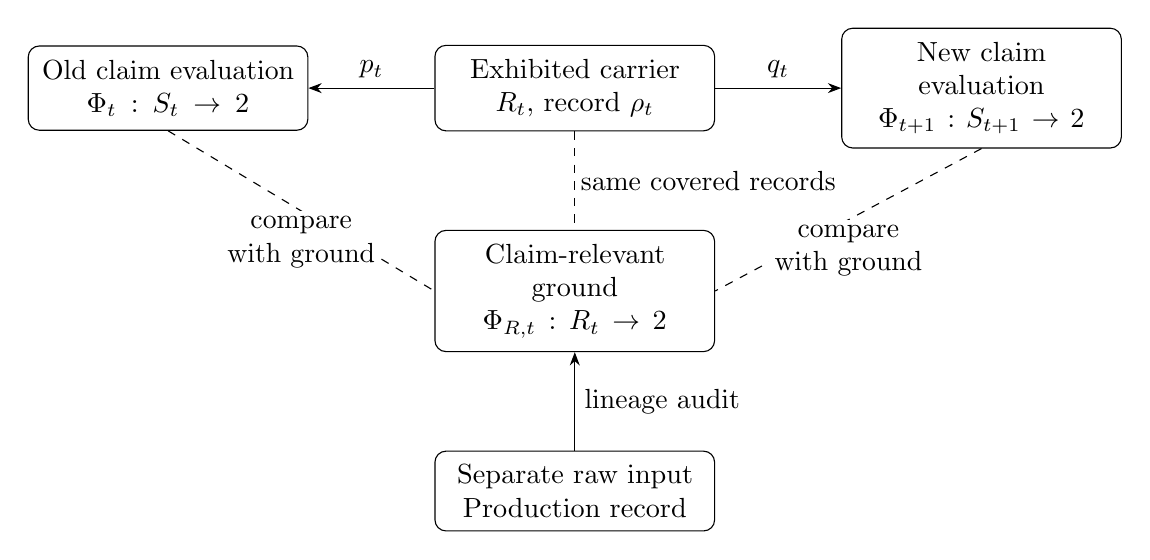
\begin{tikzpicture}[>=Stealth,node distance=1.25cm and 1.6cm,
  box/.style={draw,rounded corners,align=center,text width=3.2cm,inner sep=5pt}]
\node[box] (old) {Old claim evaluation\\$\Phi_t:S_t\to2$};
\node[box,right=of old] (carrier) {Exhibited carrier\\$R_t$, record $\rho_t$};
\node[box,right=of carrier] (new) {New claim evaluation\\$\Phi_{t+1}:S_{t+1}\to2$};
\node[box,below=of carrier] (ground) {Claim-relevant ground\\$\Phi_{R,t}:R_t\to2$};
\node[box,below=of ground] (raw) {Separate raw input\\Production record};
\draw[->] (carrier) -- node[above] {$p_t$} (old);
\draw[->] (carrier) -- node[above] {$q_t$} (new);
\draw[->] (raw) -- node[right] {lineage audit} (ground);
\draw[dashed] (carrier) -- node[right,fill=white,inner sep=2pt] {same covered records} (ground);
\draw[dashed] (old.south) -- node[midway,below,fill=white,inner sep=2pt,align=center] {compare\\with ground} (ground.west);
\draw[dashed] (new.south) -- node[midway,below,fill=white,inner sep=2pt,align=center] {compare\\with ground} (ground.east);
\end{tikzpicture}
\caption{Migration audit objects. Each endpoint needs its own observational determination evidence. Dashed links denote evaluation and comparison on the carrier; they are not production edges. Production of the ground is audited separately against (L1)--(L4).}
\label{ex:fig:audit-workflow}
\end{figure}

\begin{definition}[Seam coherence]\label{ex:def:seamcoherence}
The span is seam coherent for $(\Phi_t,\Phi_{t+1})$ when $\Phi_t \circ p_t=\Phi_{t+1} \circ q_t$.
\end{definition}

\paragraph{Engineering reading.} On every covered migrated record, the old and new claim evaluations agree. This is an endpoint-consistency test. It says nothing yet about whether the common value is correct.

\begin{definition}[Seam witness]\label{ex:def:seamwitness}
A seam witness is an element $r \in R_t$ with $\Phi_t(p_t(r)) \neq \Phi_{t+1}(q_t(r))$.
\end{definition}

\paragraph{Engineering reading.} A seam witness is one migrated record on which the old and new evaluations disagree. It is the migration analogue of a failing source--target comparison, but its subject is the declared claim rather than raw row equality.

\begin{proposition}[Span criterion]\label{ex:prop:span}
Suppose the span is seam coherent for $(\Phi_t,\Phi_{t+1})$ and $\Phi_t=\widehat\Phi_t \circ M_t$. Then $\Phi_{t+1} \circ q_t$ factors through $M_t \circ p_t$ as maps on $R_t$.
\end{proposition}

\begin{proof}
By seam coherence and the assumed factorisation,
\[
\Phi_{t+1}\circ q_t=\Phi_t\circ p_t=\widehat\Phi_t\circ M_t\circ p_t,
\]
so $\widehat\Phi_t$ is itself a factor of $\Phi_{t+1}\circ q_t$ through $M_t\circ p_t$.
\end{proof}

Proposition~\ref{ex:prop:span} establishes factorisation on $R_t$, not on all of $S_{t+1}$. It provides no information about states outside the image of $q_t$. A changed predicate needs its own certificate. The displayed factor is constructed directly and is used again in the constructive condition on later admissibility.

\subsection{Independent grounding at the seam}\label{ex:sec:grounding-seam}

Extensional seam coherence permits accidental or copied agreement. The engineering question is whether agreement between two coordinate descriptions is supported by a valuation produced from claim-relevant process evidence rather than inherited from either coordinate. Where the process can be exhibited, the assurance record therefore needs a seam valuation with a production path that can be audited independently of the two determinations it is meant to check.

Consider services $A$ and $B$ during a dual-write migration. Service $A$ emits a status line and $B$ copies it into the new-format log. Let $1$ mean ``completed without a partial effect''. On an ordinary request $r_{\mathrm{ok}}$, no partial effect occurs and the trace and both logs correctly support $1$. On request $r_*$, an irreversible side effect occurs before a failure, but $A$ prematurely writes $1$ and $B$ copies it. The execution trace supports $0$:
\[
\Phi_A(p(r_*))
=\Phi_B(q(r_*))=1,
\qquad
\Phi_R(r_*)=0,
\]
where $\Phi_R$ is evaluated from an exhibited trace. Identity evolution makes every update square commute, yet the agreement carries a false claim. Defining $\widetilde\Phi_R=\Phi_A\circ p$ would satisfy the equations only by copying the coordinate. Exhibition instead requires the continuing process, provenance from it to both coordinates, evidence sufficient to evaluate $\Phi_R$, declared coverage, and custody.

Source independence does not exhaust this requirement. Two independently maintained instruments can produce operationally independent reports and still share a blind spot because neither records a process feature on which the claim depends. Such independence may support confidence in the coordinate records without supplying a valuation of the relevant process. Grounded coherence therefore asks a different question: whether the asserted value is exhibited from claim-relevant process occurrences by a production path that runs through neither coordinate.

In the defeater vocabulary of Assurance~2.0 (Section~\ref{ex:sec:related}), a fibre witness defeats the claim that an observation surface determines the predicate; a seam witness defeats extensional transport on the exhibited carrier; a grounding witness defeats the stronger claim that the coordinate values agree with an independent process valuation. Missing carrier or lineage coverage is different again: it undercuts the inference from a clean check because the relevant case may never have entered the check. Here the record must therefore exhibit the seam valuation's production path. Conditions (L1)--(L3) below prohibit descent from either coordinate, disclose their shared derived ancestry, and require a claim-relevant raw source outside both coordinate ancestries; Section~\ref{ex:sec:laundering} adds a fourth condition on the ancestry the ground shares with them. Independence of the coordinate instruments alone would not suffice if both missed the same process feature. The delivery scan in Section~\ref{ex:sec:case} illustrates a ground that is not an ancestor of either coordinate.

Table~\ref{ex:tab:comparison} separates the claims made by different migration checks; Section~\ref{ex:sec:related} relates them to the testing literature.

\begin{table}[htbp]
\centering\small
\caption{Different claims made by migration checks. A pass in one row does not entail a pass in another.}
\label{ex:tab:comparison}
\begin{tabularx}{\textwidth}{@{}P{2.8cm}LLL@{}}
\toprule
Check & Question & Counterevidence & Positive result needs \\
\midrule
Source--target validation & Does the target match the mapped source? & Unequal mapped records & Declared mapping and checked records \\
Reconciliation & Were the declared source records accounted for? & Missing or duplicated identifiers & Independent totals and stated coverage \\
Seam coherence & Do the two claim valuations agree on the carrier? & One seam witness & Exhibited, sufficiently covered carrier \\
Grounded coherence & Do both valuations agree with a separately produced, claim-relevant seam valuation? & Grounding witness or failed lineage condition & Equations, lineage conditions, and external evidence for carrier and raw-source fidelity \\
\bottomrule
\end{tabularx}
\end{table}

A trace is also a representation. Its claim to ground the seam is defeasible: its documented path must begin in claim-relevant process occurrences and pass through neither coordinate. It may still be inaccurate or incomplete. A copied coordinate cannot establish its own agreement with another coordinate.

Some regimes cannot exhibit an independent ground. The audit then reports incomplete or obstructed lineage, not a grounding witness. If neither a ground nor a refuting witness is available, support for transport is underdetermined. The institution must obtain a new certificate, instrument future transitions, or hold the gap open as debt. It may report coordinate agreement without claiming grounded transport.

Within a migration window, write the concurrent old and new coordinate state models as $A_t$ and $B_t$:
\[
A_t\xleftarrow{p_t}R_t\xrightarrow{q_t}B_t.
\]
The carrier and projections keep the notation introduced above. $A_t$ and $B_t$ name the two schemas at window stage $t$, allowing both to evolve; they replace $S_t$ and $S_{t+1}$ only when the discussion concerns concurrent evolution rather than one consecutive cut-over. Equip $R_t$ with its record and a valuation $\Phi_{R,t}:R_t\to V_t$ from the retained process evidence. The coordinate valuations are $\Phi_{A,t}:A_t\to V_t$ and $\Phi_{B,t}:B_t\to V_t$. For the executable exact claims, $V_t=2$.

The lineage requirement is stated over a declared graph. A \emph{lineage record} for the seam is a finite directed acyclic graph $L$ whose nodes are the fields that enter the three valuations and whose edges run from each field to the fields derived from it. It declares a set $\operatorname{Raw}(L)$ of raw inputs, which enter the regime from outside it and have no incoming edges, and marks the claim-relevant raw inputs $\operatorname{Rel}(L)\subseteq\operatorname{Raw}(L)$. It contains nodes $d_A$, $d_B$, and $g$ for the determinations $\Phi_{A,t}\circ p_t$, $\Phi_{B,t}\circ q_t$, and $\Phi_{R,t}$. Write $\operatorname{anc}(x)$ for the set of strict ancestors of $x$ in $L$.


Figure~\ref{ex:fig:lineage-dag} shows the smallest pattern the three lineage clauses are meant to distinguish. A shared derived node can explain coordinate agreement without corroborating it; a separate raw process source can ground the seam valuation without descending from either coordinate.

\begin{figure}[htbp]
\centering
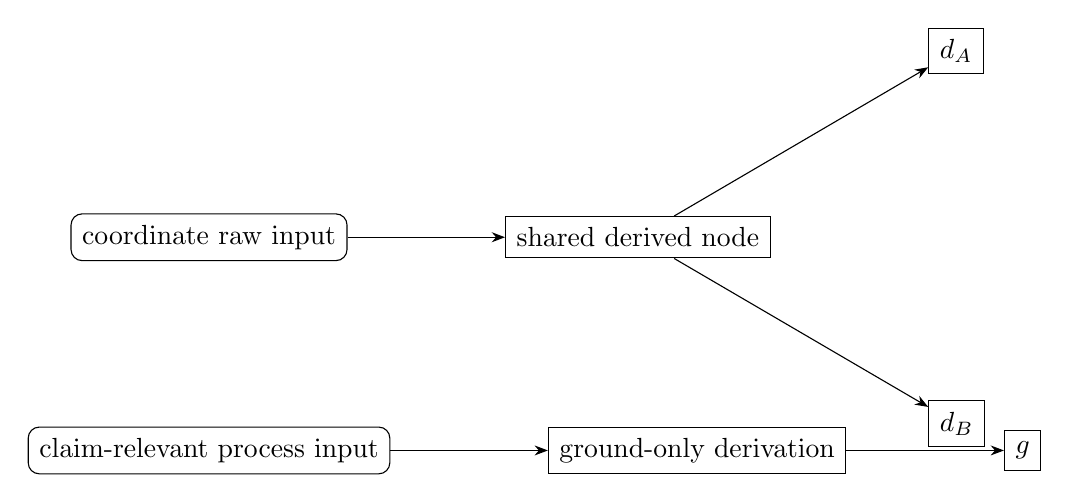
\begin{tikzpicture}[>=Stealth,node distance=1.8cm and 2.0cm,
  raw/.style={draw,rounded corners,inner sep=4pt},
  derived/.style={draw,inner sep=4pt}]
\node[raw] (coordraw) {coordinate raw input};
\node[derived, right=of coordraw] (shared) {shared derived node};
\node[derived, above right=of shared] (da) {$d_A$};
\node[derived, below right=of shared] (db) {$d_B$};
\node[raw, below=2.1cm of coordraw] (process) {claim-relevant process input};
\node[derived, right=of process] (groundmid) {ground-only derivation};
\node[derived, right=of groundmid] (g) {$g$};
\draw[->] (coordraw) -- (shared);
\draw[->] (shared) -- (da);
\draw[->] (shared) -- (db);
\draw[->] (process) -- (groundmid);
\draw[->] (groundmid) -- (g);
\end{tikzpicture}
\caption{A lineage pattern with shared coordinate ancestry and a separate claim-relevant ground. The figure is schematic: real records may contain many additional nodes and edges.}
\label{ex:fig:lineage-dag}
\end{figure}

\paragraph{Running-example bridge.} In the tax migration, the backfill route is zone $\to$ primary municipality $\to$ new tax flag. The delivery-based seam valuation instead uses the separately recorded delivery event. The point of the lineage test is not to require the new coordinate to be independent of the old one. It is to require the \emph{ground used to corroborate them} to have a claim-relevant production path that does not descend from either coordinate, while making shared coordinate ancestry explicit.

\begin{definition}[Coordinate-copied ground]\label{ex:def:copied-ground}
A proposed ground node $g$ is \emph{coordinate-copied} relative to $(d_A,d_B)$ when
\[
g=d_A\ \lor\ g=d_B\ \lor\ d_A\in\operatorname{anc}(g)\ \lor\ d_B\in\operatorname{anc}(g).
\]
This is a production-path property, not equality of reported values. Independently produced valuations can coincide without being copies. No coordinate descent (L1) is exactly the negation of this property.
\end{definition}

\begin{definition}[Three-clause lineage qualification]\label{ex:def:lineage-qualified-three}
Let the span with its record $\rho_t$ be exhibited for the claim, and let $L$ be a lineage record for the seam. The valuation $\Phi_{R,t}$ is \emph{lineage-qualified under (L1)--(L3)}, written $\operatorname{LineageQualified}_{123}(\Phi_{R,t};L)$, when
\begin{enumerate}
\item[(L1)] \emph{no coordinate descent}: $g\neq d_A$, $g\neq d_B$, $d_A\notin\operatorname{anc}(g)$, and $d_B\notin\operatorname{anc}(g)$;
\item[(L2)] \emph{shared ancestry disclosure}: the record lists the shared non-raw ancestry $D=(\operatorname{anc}(d_A)\cap\operatorname{anc}(d_B))\setminus\operatorname{Raw}(L)$ and enters each element of $D$ either with a justification or as an open defeater to inference from coordinate agreement;
\item[(L3)] \emph{independent raw source}: the ground-only source set
\[
G=\bigl(\operatorname{anc}(g)\cup\{g\}\bigr)\setminus
\bigl(\operatorname{anc}(d_A)\cup\operatorname{anc}(d_B)\cup\{d_A,d_B\}\bigr)
\]
contains at least one claim-relevant raw input: $G\cap\operatorname{Rel}(L)\neq\emptyset$.
\end{enumerate}
\end{definition}

\paragraph{Engineering reading of (L1)--(L3).} (L1) says that the corroborating ground must not be the old or new determination and must not have been derived from either of them. It is a condition on the ground, not a prohibition on the target field being copied during a migration. (L2) says to list shared derived dependencies of the two coordinates, such as a common zone lookup or upstream service, and record whether each dependency has been answered or remains an open defeater. (L3) says that the ground must have at least one claim-relevant raw source outside both coordinate ancestries. In the running example the delivery event plays that role. A new municipality backfilled from the old zone can therefore be audited, but it cannot serve as its own corroboration.

\paragraph{A three-source example.} Let a raw address $a$ produce a derived zone $z$, with $z\to d_A$ and $z\to d_B$, while a separate claim-relevant raw delivery event $h$ produces $g$. Then no coordinate descends into $g$, so (L1) passes. The shared non-raw ancestor set is $D=\{z\}$, so (L2) requires a disposition for $z$. The event $h$ is outside both coordinate ancestries and witnesses (L3). Leaving $z$ as an open defeater satisfies disclosure without resolving the concern. Replacing the delivery-based ground by $d_A\to g$ makes it coordinate-copied and fails (L1), even if its numerical output remains unchanged.

Claim relevance is a declaration attached to a raw input for the specified claim. The structural audit checks that the input is declared, raw, consistently marked, and in the required ground-only set. It does not prove that the marking is true or that the instrument captured the relevant occurrence faithfully.

The clauses prevent three different errors. Since ancestry is strict, the explicit inequalities in (L1) exclude the degenerate case in which the purported ground is a coordinate node itself. The absence of each coordinate from $\operatorname{anc}(g)$ excludes any directed dependency path from that coordinate to the ground. (L2) exposes shared derived ancestry that could explain agreement without corroboration. The inclusion of $g$ in (L3) permits a direct raw process input to serve as the ground; its exclusion from both coordinate ancestries still has to be checked. Each clause can fail while the other two hold. A relevant raw input that appears only on one route is a necessary graph condition, not a proof that the recorded route exhausts the actual production of the valuation.

\paragraph{Implementation scope.}
The current Paper 2A decision core reflects (L1)--(L4); the companion has its own three-clause checker. Their guarantees and tests have separate attribution (Appendix~\ref{ex:app:mechanisation}). Historical differences in identity and directly raw ground handling are retained in Appendix~\ref{ex:app:history}. Neither checker establishes source use, evaluator validity or clearance.

\paragraph{Structural passing and certificate issuance.}
Conditions (L2) and (L4) are disclosure conditions. Recording a shared ancestor as an open defeater satisfies disclosure but does not discharge the concern. A structural pass under (L1)--(L4) therefore does not by itself license an unqualified transport certificate. Issuance additionally requires all declared defeaters to be resolved and the declared coverage to have no outstanding gaps, as well as the remaining transport obligations. These resolution and coverage requirements are separate from (L2) and (L4). They preserve the difference between an accurate record of a concern and evidence that answers it.

\paragraph{Adversarial and incomplete records.} The custodian of Definition~\ref{ex:def:exhibited-seam} holds $L$. Passing (L1)--(L4) checks the declared derivation, not the graph's completeness or the raw source's accuracy, and an omitted production path may defeat the assurance (Section~\ref{ex:sec:case-audit}). A fabricated graph can satisfy the syntax while misdescribing production, and a materially incomplete one can hide descent from a coordinate. The threats are concrete: an operator may omit failed writes to meet a cut-over target, a backfill service may label a copied zone lookup as geocoded, a compromised producer may emit false source events, or a later custodian may remove a dependency that reveals copying. Distinct controls address distinct opportunities. Binding lineage records to source and deployment identifiers and reconciling declared paths against independently held totals challenge omission; authenticated, tamper-evident event capture makes later alteration detectable; and independent validation of a sample challenges a false value at capture. Cryptographic integrity can protect a recorded history from later alteration; it cannot establish that the history was complete or truthful when created. The assurance record should name the producer of each lineage edge, the retention and access controls, and any portion for which independent corroboration is unavailable.

\paragraph{Binding is necessary but not grounding.}
A certificate, proposal, or migration record can be internally valid and still be attached to the wrong assertion. A transport record should therefore bind the claim, the old and new versions, the computed coordinate statuses, the seam record, and the lineage result that is asserted about them. Where possible, the downstream record should be constructed from those actual objects rather than accept a caller-supplied certificate whose subject is merely assumed to match. This prevents one claim's warrant record from being substituted for another. It does not establish independent ground. A perfectly bound certificate can still certify a value copied from one coordinate, and two correctly bound records can still share one production source. Claim binding and lineage independence are separate obligations.

The graph need not be stored in the paper's bespoke notation. A deployment can encode raw observations and derived records as PROV entities, transformations as activities, and responsible services or people as agents \citep{w3cprovdm2013}; derivation edges then supply the ancestry relation used by the audit. PROV records a declared history; it does not by itself guarantee that the history is complete, that a source is claim-relevant, or that two records are independent in the sense required here.

For relational queries, provenance-semiring annotations can preserve alternatives and joint dependencies that a simple edge list may flatten \citep{greenkarvounarakistannen2007}. Conditions (L1)--(L4) apply to them only after an explicit account maps annotations and transformation steps to the distinguished valuations and declares the relevant raw sources; the occurrence of a coordinate variable in one derivation differs from its being a factor of every derivation. No such mapping is implemented here.

A partial lineage record can support only a coverage-qualified result. The record must mark the nodes, transformations, versions, and transition interval it covers; any unrecorded claim-relevant segment remains an open construction obligation, and the audit must report ``pass relative to $L$'' together with the gap rather than global lineage grounding. Where several candidate grounds $g_1,\ldots,g_k$ exist, each candidate is audited separately against (L1)--(L4) and its own coverage. One candidate suffices only for the seam elements and claim for which it is exhibited and claim-relevant. Combining partial grounds requires an explicit aggregation map and a coverage argument; distinct field names do not establish independence, and shared ancestry among the grounds must itself be declared. If no candidate covers the asserted transition, transport remains underdetermined even when every audited fragment passes.

For an incomplete legacy source, the custodian inventories the surviving schemas, writes, versions, and independent traces, marking the interval and claims each covers. A reconstructed path is entered as an inference, never a raw observation. A sample can challenge a proposed mapping but cannot certify an unreachable remainder. The audit returns a counterexample, a pass relative to a bounded graph, or an obstruction of the required history. The institution must then narrow the transport claim, obtain new evidence, or operate with marked debt. Obstruction establishes no fact about the missing path.

\subsection{Grounds that launder shared ancestry}\label{ex:sec:laundering}

Condition (L1) forbids the ground from descending from the coordinate determinations, but not from their ancestors. A ground can therefore pass (L1)--(L3) while reading a derived node that also feeds both coordinates.

\begin{proposition}[Laundering through shared ancestry]\label{ex:prop:laundering}
There is an exhibited seam with a lineage record satisfying (L1)--(L3) whose seam valuation is a function of a derived node shared by both coordinates, satisfies both grounding equations, and is false at a seam record.
\end{proposition}
\begin{proof}
Use the dual-write services example of Section~\ref{ex:sec:grounding-seam}: the carrier $R=\{r_{\mathrm{ok}},r_*\}$ is exhibited by the two request identifiers, their old and new log entries, the execution trace, coverage $C=R$, and a declared custodian; both coordinate valuations equal $1$ at both records; and the trace records a partial effect at $r_*$. Take raw nodes $a,h$, derived nodes $s,d_A,d_B,g$, and the edges
\[
a\to s,\qquad s\to d_A,\qquad s\to d_B,\qquad s\to g,\qquad h\to g,
\]
with $s$ the shared status line, $h$ the trace, and $\operatorname{Rel}(L)=\{h\}$. Then $\operatorname{anc}(g)=\{a,s,h\}$ contains neither coordinate, and $g$ differs from both, so (L1) holds. The shared non-raw coordinate ancestry is $D=\{s\}$, which can be disclosed, so (L2) holds. The ground-only set is $\{h,g\}$, which contains the claim-relevant $h$, so (L3) holds. Let the seam valuation be the recorded status line, $\Phi_R(r)=v_s(r)$, which is $1$ at both records. Both grounding equations $\Phi_A\circ p=\Phi_R=\Phi_B\circ q$ hold, yet the trace shows that the claim fails at $r_*$.
\end{proof}

The proposition exposes two gaps at once. (L1) does not look upstream of the coordinates, and (L3) asks only that a claim-relevant source be present in the ground's ancestry, not that the valuation use it. Here $h$ is present and ignored.

\begin{definition}[Shared ground ancestry and disclosure]\label{ex:def:separation}
For a lineage record $L$ with distinguished nodes $d_A,d_B,g$, let
\[
E_g=\bigl(\operatorname{anc}(g)\cap(\operatorname{anc}(d_A)\cup\operatorname{anc}(d_B))\bigr)\setminus\operatorname{Raw}(L)
\]
be the derived ancestry that the ground shares with either coordinate. The record satisfies
\begin{enumerate}
\item[(L4)] \emph{ground-ancestry disclosure} when it lists $E_g$ and enters each element either with a justification or as an open defeater to inference from agreement with the ground.
\end{enumerate}
The ground is \emph{strictly separated} when $E_g=\emptyset$. Condition (L4) establishes ground-ancestry disclosure; disclosure alone establishes no separation.
\end{definition}

\begin{definition}[Lineage qualification and clearance]\label{ex:def:lineage-qualified}
An exhibited seam valuation is \emph{lineage-qualified} by $L$, written $\operatorname{LineageQualified}(\Phi_{R,t};L)$, when $\operatorname{LineageQualified}_{123}(\Phi_{R,t};L)$ and (L4) hold. This is the structural (L1)--(L4) status. It can hold with disclosed defeaters still open.

For a declared claim and scope $C$, it is \emph{lineage-cleared}, written $\operatorname{LineageCleared}(\Phi_{R,t};L,C)$, when it is lineage-qualified, evidence resolves the declared lineage defeaters, no claim-relevant lineage-coverage gap remains within $C$, and a ground-evaluator justification is recorded. This justification identifies the implemented computation and its evidence inputs, supports its evaluation of the declared claim on $C$, and explains the claim-bearing use of the independent source required by (L3). The presence, availability or syntactic reading of that source is insufficient. An independent input need not change every answer, but its contribution to the claimed corroboration must be evidenced.

Clearance and ground-evaluator justification are assurance judgements. They remain conditional on model relevance and raw-source fidelity; neither is established by the graph check or by a justification string. The predicate $\operatorname{GroundEvaluatorJustified}(\rho_t;\chi,C)$ below names this recorded obligation. The runtime checker does not decide it.
\end{definition}

(L4) permits the ground to share raw inputs with the coordinates, such as a charged rate or a published rate table, which a valuation of the same claim will often need. It requires every shared \emph{derived} input to be named. Like (L2), it is a disclosure condition: an open (L4) defeater satisfies the structural condition and blocks issuance. In Proposition~\ref{ex:prop:laundering}, $E_g=\{s\}$, so the laundered ground passes (L4) only by recording the status line as an open defeater or by justifying it.

Where a justification asserts that retained shared ancestry does not determine the ground, the fibre criterion supplies a finite test of that extensional assertion. Suppose the record retains, for each seam element $r$, the tuple $v_E(r)$ of values recorded at the nodes of $E_g$.

\begin{proposition}[A fibre test for laundering]\label{ex:prop:laundering-test}
$\Phi_{R,t}$ is $v_E$-admissible on $R_t$ if and only if there is no pair $r,r'\in R_t$ with $v_E(r)=v_E(r')$ and $\Phi_{R,t}(r)\neq\Phi_{R,t}(r')$.
\end{proposition}
\begin{proof}
Lemma~\ref{ex:prop:fibre}, in its nonempty-codomain form, with $R_t$ for $S$, $v_E$ for $M$, and $\Phi_{R,t}$ for $\Phi$.
\end{proof}

If the ground is $v_E$-admissible, its retained values factor through the retained shared-ancestry values on the exhibited carrier. This is an extensional result on those records; it does not establish how the ground was actually produced. The clean test supplies no separation witness with which to resolve a nonempty shared-derived-ancestry concern, so that concern remains open unless other evidence answers it. A witness pair establishes that the retained ground distinguishes records the retained shared ancestry identifies. It refutes that factorisation, but does not prove causal independence, substantive use of the (L3) source, or its fidelity. A genuinely independent source can also happen to agree everywhere on a restricted carrier; the test does not thereby prove copying. In Proposition~\ref{ex:prop:laundering}, the laundered valuation $\Phi_R=v_s$ is trivially $v_s$-admissible. Had the trace valuation been recorded with the same edge $s\to g$, the pair $(r_{\mathrm{ok}},r_*)$, which agrees on the status line and differs on the trace, would refute $v_s$-admissibility. On a finite carrier the test is the reference procedure of Section~\ref{ex:sec:finite-procedure} with $v_E$ as the observation map. Where the record does not retain the values of the shared nodes, the defeater cannot be resolved this way and remains open.

\begin{proposition}[Shared raw input and an ignored independent source]\label{ex:prop:raw-source-bypass}
There is an exhibited seam whose ground satisfies (L1)--(L4), strict derived-ancestry separation and both grounding equations, but does not evaluate the declared claim correctly.
\end{proposition}
\begin{proof}
Take the two-record carrier $R=\{r_{\mathrm{ok}},r_*\}$, with stable identifiers, both coordinate records, retained raw inputs, complete declared coverage and a custodian. Let the raw input $a$ record request arrival, with value $1$ at both records. Let a separate claim-relevant raw input $h$ faithfully record whether the request completed without a partial effect, with values $1$ and $0$ respectively. Both retained inputs can be faithful to what they record.

Take derived nodes $d_A,d_B,g$, raw nodes $a,h$, relevance set $\{h\}$ and edges
\[
a\to d_A,\qquad a\to d_B,\qquad a\to g,\qquad h\to g.
\]
The proposed ground reads the available inputs but returns $a$, ignoring $h$. Thus
\[
\operatorname{anc}(d_A)=\operatorname{anc}(d_B)=\{a\},
\qquad\operatorname{anc}(g)=\{a,h\}.
\]
No coordinate equals or precedes $g$, so (L1) holds. Shared coordinate ancestry is raw, so $D=\emptyset$ and (L2) is vacuous. The ground-only set is $G=\{h,g\}$, giving (L3). Since all ancestry shared with the ground is raw, $E_g=\emptyset$; (L4) and strict separation hold. Assign both coordinate valuations and $\Phi_R$ the value of $a$. Both grounding equations hold on all of $R$, but the declared no-partial-effect claim fails at $r_*$, as the faithful input $h$ records.
\end{proof}

This is a limitation of the graph specification, not an omitted edge or inaccurate source. The graph records an available source without establishing its claim-bearing use. Conditions (L1)--(L4) can therefore expose certain dependencies without certifying the ground's evaluator, even when $D=E_g=\emptyset$. Ground-evaluator justification fails in this countermodel. The recorded absence of open derived-ancestry defeaters cannot substitute for that obligation. The Coq examples and the executable control are mapped in Appendix~\ref{ex:app:v18-verification}.

\begin{remark}[Injective retained ancestry]\label{ex:rem:injective-ancestry}
If $v_E$ is injective on the exhibited carrier, every ground valuation factors through it: its fibres are singletons. A complete finite check then returns a factor, irrespective of the valuation's production path. In particular, a shared derived identifier that uniquely identifies every record can prevent the fibre test from supplying any separation witness. This is not evidence of copying or of independence.

Each diagnostic should state the suspected dependency, the retained observation tuple and the carrier on which the factorisation claim is tested. Testing a selected subset of shared nodes names a different obligation; a witness against that subset does not refute dependence on the full tuple. The source-use and evaluator justification must address whatever the finite test leaves unresolved. The extension proves the injective-observation limit constructively and exercises it in the runtime controls.
\end{remark}

\subsection{Grounded seam coherence}\label{ex:sec:grounded-coherence}

\begin{definition}[Grounded seam coherence]\label{ex:def:grounded-seam}
Let $A_t \xleftarrow{p_t} R_t
\xrightarrow{q_t} B_t$ be a seam, with valuations
$\Phi_{A,t}:A_t\to V_t$, $\Phi_{B,t}:B_t\to V_t$, and
$\Phi_{R,t}:R_t\to V_t$. The seam is \emph{groundedly coherent} when (a) the span with its record $\rho_t$ is exhibited for the claim (Definition~\ref{ex:def:exhibited-seam}); (b) the record contains a lineage record $L$ by which $\Phi_{R,t}$ is lineage-qualified under (L1)--(L4) (Definition~\ref{ex:def:lineage-qualified}); and (c) the grounding equations hold:
\[
\Phi_{A,t}\circ p_t
=\Phi_{R,t}
=\Phi_{B,t}\circ q_t.
\]
Equivalently, for every $r\in R_t$,
\[
\Phi_{A,t}(p_t(r))
=\Phi_{R,t}(r)
=\Phi_{B,t}(q_t(r)).
\]
\end{definition}

\paragraph{Engineering reading.} A structural grounded-coherence pass requires an auditable migration population, a claim-relevant valuation with lineage qualification, and equality of both coordinate evaluations with that valuation on every covered record. Any disclosed defeater remains open until clearance is separately recorded. Merely matching old and new outputs satisfies only the last comparison between the coordinates.

\begin{table}[htbp]
\centering\small
\caption{Levels of a migration claim. Every result retains its declared claim and coverage.}
\label{ex:tab:claim-levels}
\begin{tabularx}{\textwidth}{@{}P{3.1cm}LL@{}}
\toprule
Status & Formal obligation & Record and institutional obligation \\
\midrule
Lineage-qualified & (L1)--(L4) pass on the declared graph & Exhibited valuation and source declarations; open (L2) and (L4) defeaters remain open \\
Lineage-cleared & Lineage-qualified & Declared lineage defeaters resolved, lineage coverage closed and ground evaluator justified for the claim and scope; source fidelity remains a premise \\
Groundedly coherent & Lineage-qualified ground and both grounding equations & Exhibited span and record; evaluator validity, carrier coverage and source fidelity remain separate obligations \\
Structurally transportable & Grounded coherence, inhabited carrier, endpoint admissibility, functorial evolution & Evidence bound to the same claim and declared interval \\
Transportable for issuance & All structural obligations established & Declared defeaters and coverage gaps resolved; ground evaluator justified; maintained evidence and authorised custody for the claim and use \\
\bottomrule
\end{tabularx}
\end{table}

Grounded coherence is the structural status defined above; it can coexist with an unresolved disclosed lineage concern. It implies coordinate agreement. The converse fails: a valuation copied from one coordinate can satisfy the equations while failing lineage condition (b). The extra structure makes the proposed ground inspectable; it does not establish that the carrier adequately represents the process.

\begin{proposition}[Grounding entails extensional seam coherence]\label{ex:prop:grounding-entails-coherence}
Every groundedly coherent seam is seam coherent in the sense of Definition~\ref{ex:def:seamcoherence}.
\end{proposition}

\begin{proof}
For every $r\in R_t$, both
$\Phi_{A,t}(p_t(r))$ and
$\Phi_{B,t}(q_t(r))$ are equal to
$\Phi_{R,t}(r)$.
\end{proof}

\begin{definition}[Grounding witness]\label{ex:def:grounding-witness}
A grounding witness for a seam with an exhibited, lineage-qualified valuation $\Phi_{R,t}$ is an element $r\in R_t$ with $\Phi_{A,t}(p_t(r))\neq\Phi_{R,t}(r)$ or $\Phi_{B,t}(q_t(r))\neq\Phi_{R,t}(r)$.
\end{definition}

\paragraph{Engineering reading.} This is the row that an endpoint comparison can miss. Either endpoint disagrees with the separately produced ground. The two endpoints may still agree with each other. The running row $(2,5,\mathit{general},\mathit{before},60)$ is exactly that case: the copied flags agree, while the delivery-based valuation disagrees.

Read on the carrier $R_t$, every seam witness in the sense of Definition~\ref{ex:def:seamwitness} is a grounding witness, because two coordinate values that differ cannot both equal $\Phi_{R,t}(r)$. The converse fails, and its failure is the point of the grounded condition: at a grounding witness the two coordinates may agree with each other while both depart from the process. A single grounding witness refutes grounded coherence, as a single seam witness refutes extensional coherence; the checked lemmas are identified in Appendix~\ref{ex:app:verification}.

\begin{proposition}[Ungrounded agreement]\label{ex:prop:ungrounded-agreement}
There exist exhibited spans whose coordinate predicates satisfy extensional seam coherence and whose identity update maps satisfy functorial commutation, but for which grounded coherence fails: the lineage-qualified process valuation disagrees with both coordinates, and the valuation that agrees with them fails the lineage condition. Such a span can transport a false claim.
\end{proposition}

\begin{proof}
Let $R=\{r_{\mathrm{ok}},r_*\}$, $A=\{a_{\mathrm{ok}},a_*\}$, and $B=\{b_{\mathrm{ok}},b_*\}$. Define $p(r_i)=a_i$ and $q(r_i)=b_i$, and let both coordinate predicates be constantly $1$. Thus $\Phi_A\circ p=\Phi_B\circ q$ on all of $R$. Repeat these sets and maps at every stage and take all update maps to be identities. Both naturality squares, the identity laws, and the composition laws then hold directly. Identity evolution makes these checks vacuous with respect to change; it supplies no grounding evidence.

Exhibit the two request identifiers, their old and new log entries, the execution trace, coverage $C=R$, and a declared custodian in $\rho$. The trace valuation is $\Phi_R(r_{\mathrm{ok}})=1$ and $\Phi_R(r_*)=0$: at $r_*$ it records the partial effect missed by the status line. These declarations satisfy the five exhibition conditions in this finite countermodel.

For lineage, take raw nodes $a,h$, derived nodes $s,d_A,d_B,g$, and exactly the edges
\[
a\to s,\qquad s\to d_A,\qquad s\to d_B,\qquad h\to g.
\]
Here $s$ is the shared status line, $h$ is the claim-relevant trace, and $\operatorname{Rel}(L)=\{h\}$. The graph is acyclic. Its strict ancestor sets are
\[
\operatorname{anc}(d_A)=\operatorname{anc}(d_B)=\{a,s\},
\qquad \operatorname{anc}(g)=\{h\}.
\]
The three distinguished nodes are distinct, and neither coordinate is an ancestor of $g$, so (L1) holds. The shared non-raw set is $D=\{s\}$; disclosing $s$ as an open defeater satisfies (L2). The ground-only set is $G=\{h,g\}$, so $G\cap\operatorname{Rel}(L)=\{h\}$ and (L3) holds. Since $\operatorname{anc}(g)=\{h\}$ shares nothing with the coordinates, $E_g=\emptyset$ and the ground is strictly separated. This proves lineage qualification without an executable audit. At $r_*$, however, both coordinate values are $1$ and $\Phi_R(r_*)=0$. The grounding equations fail, so grounded coherence fails despite endpoint equality and functorial commutation.

For the agreeing alternative, add a fresh node $\widetilde g$ with the single incoming edge $d_A\to\widetilde g$ and valuation $\widetilde\Phi_R=\Phi_A\circ p$. It is constantly $1$, so both grounding equations hold. But $d_A\in\operatorname{anc}(\widetilde g)$, violating (L1). Also
\[
\operatorname{anc}(\widetilde g)=\{a,s,d_A\},
\qquad \widetilde G=\{\widetilde g\},
\]
and $\widetilde G\cap\operatorname{Rel}(L)=\emptyset$, violating (L3). Thus the valuation that matches the endpoints is coordinate-copied, while the lineage-qualified valuation refutes their common claim. The record $r_*$ is a grounding witness and is not a seam witness.
\end{proof}

Coq checks the equational part with \code{copied\_\allowbreak not\_\allowbreak grounded} and \code{grounding\_\allowbreak witness\_\allowbreak refutes}. The five OCaml case-study records exercise the historical lineage audit within the scope stated in Section~\ref{ex:sec:case-audit}; the paper proof does not depend on executing them.

The practical consequence is that the assurance record must contain the ground and its production path, not only the two coordinate values.

\section{Evolution and composition}\label{ex:sec:evolution}

\subsection{Functorial transport}\label{ex:sec:functorial-transport}

For a data engineer, the question in this subsection is whether multi-stage updates preserve the same record relationships when the seam, old coordinate, and new coordinate all evolve. Checking one cut-over pair is not enough if a longer migration is certified by composing several stages.

Grounding at one stage does not constrain evolution. For stages $t\leq u$, let the seam and its coordinates evolve from $t$ to $u$ by
$U^{R}_{t,u}:R_t\to R_u$, $U^{A}_{t,u}:A_t\to A_u$, and $U^{B}_{t,u}:B_t\to B_u$. The persistence of the seam process must determine the persistence of its coordinate descriptions, which requires the squares
\begin{equation}\label{ex:eq:dynamic-squares}
\begin{tikzcd}[column sep=large,row sep=large,baseline=(current bounding box.center)]
R_t \arrow[r,"U^{R}_{t,u}"] \arrow[d,"p_t"']
  & R_u \arrow[d,"p_u"] \\
A_t \arrow[r,"U^{A}_{t,u}"'] & A_u
\end{tikzcd}
\qquad
\begin{tikzcd}[column sep=large,row sep=large,baseline=(current bounding box.center)]
R_t \arrow[r,"U^{R}_{t,u}"] \arrow[d,"q_t"']
  & R_u \arrow[d,"q_u"] \\
B_t \arrow[r,"U^{B}_{t,u}"'] & B_u
\end{tikzcd}
\end{equation}
to commute:
\begin{align}
p_{u}\circ U^R_{t,u} &=U^A_{t,u}\circ p_{t},\label{ex:eq:back-naturality}\\
q_{u}\circ U^R_{t,u} &=U^B_{t,u}\circ q_{t}. \label{ex:eq:fwd-naturality}
\end{align}
These are naturality conditions: the projections are natural transformations from the seam evolution to the coordinate evolutions. Their content is that a process cannot acquire incompatible histories because two architectural descriptions were evolved independently. The evolution maps must also satisfy, for $X \in \{R,A,B\}$ and stages $t\leq u\leq v$,
\begin{align}
U^{X}_{t,t} &=\operatorname{id}_{X_t},\label{ex:eq:evolution-identity}\\
U^{X}_{t,v} &=U^{X}_{u,v}\circ U^{X}_{t,u},\label{ex:eq:evolution-composition}
\end{align}
so that each assignment $t \mapsto X_t$, $(t\leq u)\mapsto U^X_{t,u}$ is a functor from the ordered set $(T,\leq)$, regarded as a category, to the category of sets. Without Equation~\eqref{ex:eq:evolution-composition}, the map used for a long migration could differ from the composite of its certified parts.

\begin{proposition}[Commutation composes]\label{ex:prop:commutation-composes}
If the squares commute for $t\to u$ and $u\to v$, and Equations~\eqref{ex:eq:evolution-identity} and~\eqref{ex:eq:evolution-composition} hold, the squares commute for $t\to v$.
\end{proposition}

\begin{proof}
For every $r \in R_t$,
\begin{align*}
p_v(U^R_{t,v}(r))
&=p_v(U^R_{u,v}(U^R_{t,u}(r)))
=U^A_{u,v}(p_u(U^R_{t,u}(r)))\\
&=U^A_{u,v}(U^A_{t,u}(p_t(r)))
=U^A_{t,v}(p_t(r)).
\end{align*}
The forward case replaces $A$ and $p$ by $B$ and $q$.
\end{proof}

Grounded coherence is synchronic and functorial commutation is diachronic. Neither requires the valuation to stay unchanged. If the value spaces carry a transport $U^V_{t,u}$, one may add $\Phi_{R,u} \circ U^R_{t,u}=U^V_{t,u} \circ \Phi_{R,t}$; without such a transport, requiring $\Phi_{R,u} \circ U^R_{t,u}=\Phi_{R,t}$ would turn a dynamic predicate into a temporal invariant.

\paragraph{Claims and their implementations.} The transport definition below needs one more distinction. Let $\chi$ be the declared claim of Definition~\ref{ex:def:coverage}, and write $\chi_t:S_t\to2$ and $\chi_{t+1}:S_{t+1}\to2$ for its evaluation on the two stage models; that each stage model represents the claim-relevant occurrence is a relevance obligation. The coordinate predicates $\Phi_t$ and $\Phi_{t+1}$ are the institution's implementations of $\chi$, and the seam valuation $\Phi_{R,t}$ evaluates $\chi$ from process evidence. In the cut-over reading $A_t=S_t$ and $B_t=S_{t+1}$, so that $\Phi_{A,t}=\Phi_t$ and $\Phi_{B,t}=\Phi_{t+1}$. A certificate that $\Phi_t$ is admissible on $M_t$ is a fact about $\Phi_t$. It bears on $\chi$ only where $\Phi_t=\chi_t$ on the certified scope; otherwise it certifies a different claim, and the gap is a relevance defect rather than an admissibility pass. The endpoint conjuncts of transport are therefore stated for $\chi$.

\begin{definition}[Structural transport and certificate issuance]\label{ex:def:nonvacuous-transport}
The claim $\chi$ is structurally transportable from $t$ to $t+1$ over the declared interval when
\[
\begin{aligned}
\operatorname{StructuralTransport}_{t,t+1} \Longleftrightarrow{}&
\operatorname{Inhabited}(R_t) \land \operatorname{Exhibited}(\rho_t) \\
&{}\land \operatorname{LineageQualified}(\Phi_{R,t};L_t) \\
&{}\land \operatorname{Admissible}_{M_t}(\chi_t) \land \operatorname{Admissible}_{M_{t+1}}(\chi_{t+1}) \\
&{}\land \operatorname{GroundingEquations}_t \land \operatorname{Functorial}(U;I_t).
\end{aligned}
\]
Certificate issuance additionally requires
\[
\begin{aligned}
\operatorname{Transportable}_{t,t+1}(C)\Longleftrightarrow{}&
\operatorname{StructuralTransport}_{t,t+1}\\
&{}\land\operatorname{DefeatersResolved}(\rho_t,L_t;C)\\
&{}\land\operatorname{CoverageClosed}(\rho_t,L_t;C)\\
&{}\land\operatorname{GroundEvaluatorJustified}(\rho_t;\chi,C)\\
&{}\land\operatorname{CurrentEvidenceAndCustody}(\rho_t;C).
\end{aligned}
\]
The latter predicates name assurance obligations recorded for the claim, use, time, and scope $C$, not new mechanically proved properties of the concrete process.
\end{definition}

Definition~\ref{ex:def:nonvacuous-transport} separates the structural obligations from the assurance obligations for issuance. Section~\ref{ex:sec:pcfw} states how checked endpoint evidence may discharge the observational conjuncts. The remaining conjuncts need their own evidence. Read operationally, the definition is a sequence rather than an opaque conjunction. First confirm that some process element actually crosses the interval. Second exhibit the carrier and its coverage. Third audit the lineage of the proposed ground. Fourth establish static admissibility at both endpoints. Fifth test the grounding equations on the seam. Sixth check naturality, identity, and composition over the declared interval. A failure stops the transport claim at that stage; later checks may still be diagnostically useful, but they do not repair the failed obligation.

Here $R_t$ is the carrier of the span exhibited by $\rho_t$, $L_t$ is its lineage record, and the grounding-equation conjunct is the pair of equations in condition (c) of Definition~\ref{ex:def:grounded-seam}. The exhibition, lineage and separation, and equation conjuncts are conditions (a), (b), and (c) of that definition, listed separately so that each can be assessed and reported on its own; together they are grounded coherence. The Coq development uses the same name for the equational conjunct alone. The functoriality conjunct is a property of the whole family of evolution maps $U=\{U^X_{u,v}\mid X\in\{R,A,B\},\ u\leq v,\ u,v\in I_t\}$ over the declared interval $I_t\subseteq T$, not of a single transition: every naturality square in Equations~\eqref{ex:eq:back-naturality} and~\eqref{ex:eq:fwd-naturality} commutes, and Equations~\eqref{ex:eq:evolution-identity} and~\eqref{ex:eq:evolution-composition} hold, for all composable stages in $I_t$. The conjuncts separate non-vacuity, evidence, lineage, static sufficiency, grounding, and temporal structure. An empty seam satisfies the universal equations vacuously and transports nothing; if no process continues through the interval, any later assertion requires a new certificate. A seam whose carrier and projections are not exhibited has not had its coherence disproved, but that coherence is unauditable and supplies no warrant. If the observation surface itself changes from $O_t$ to $O_{t+1}$ and coherence is asserted at the observational level, an explicit translation between surfaces is also required (Section~\ref{ex:sec:debt-extensions}). The obligation is not specific to software: wherever separately updated coordinate models describe one declared process, the same squares state what it means for them to remain its projections.

\emph{DefeatersResolved} requires evidence answering each declared open concern rather than merely recording it. \emph{CoverageClosed} requires evidence or an explicit narrowing of $C$ for outstanding carrier and lineage gaps within the assertion's scope. \emph{GroundEvaluatorJustified} records the evaluator and independent-source justification of Definition~\ref{ex:def:lineage-qualified}; a faithful input with an inadequate or source-ignoring evaluator does not discharge it. \emph{CurrentEvidenceAndCustody} records continued adequacy, evidence retention, and authorised responsibility. Each may be inspected or challenged; none is established by the structural conjunction alone. These issuance predicates are specifications for the assurance record, not mechanised definitions.

The claim that an audit covered a transition needs an assurance procedure outside the checker, and three completeness questions must be kept separate: whether the state model contains the distinctions relevant to the claim, whether the seam carrier covers the asserted interval, and whether the lineage record captures the production paths actually used. The carrier declaration should list state and transition types, source systems and versions, date range, inclusion and exclusion predicates, record counts, deduplication rules, and missing or failed extracts, and the custodian should reconcile those counts against independent source totals where available. Sampling and reconciliation can expose omissions but do not prove an unreachable remainder complete. An adjudicator need not replay a Coq proof to challenge coverage: they need the signed carrier declaration, a readable account of how records entered it, a comparison with independently held totals or samples, and a route to demand missing categories.

\subsection{Composition of seams}\label{ex:sec:lineage-composition}

A long migration is often certified step by step. Proposition~\ref{ex:prop:commutation-composes} shows that commutation composes; this subsection asks the same question of grounding. Let consecutive seams $A_0\xleftarrow{p_{01}}R_{01}\xrightarrow{q_{01}}A_1$ and $A_1\xleftarrow{p_{12}}R_{12}\xrightarrow{q_{12}}A_2$ share the middle coordinate, and form the composite carrier
\[
R_{02}=R_{01}\times_{A_1}R_{12}=\{(r,r')\in R_{01}\times R_{12}\mid q_{01}(r)=p_{12}(r')\},
\]
with projections $p_{02}(r,r')=p_{01}(r)$ and $q_{02}(r,r')=q_{12}(r')$.

\begin{proposition}[Grounding equations compose]\label{ex:prop:equations-compose}
Let $\Phi_i:A_i\to V$ for $i=0,1,2$, and suppose both seams satisfy their grounding equations with the same middle valuation $\Phi_1$. Then $\Phi_{R,01}(r)=\Phi_{R,12}(r')$ for every $(r,r')\in R_{02}$, and $\Phi_{R,02}(r,r')=\Phi_{R,01}(r)$ satisfies $\Phi_0\circ p_{02}=\Phi_{R,02}=\Phi_2\circ q_{02}$.
\end{proposition}
\begin{proof}
For $(r,r')\in R_{02}$,
\[
\Phi_0(p_{01}(r))=\Phi_{R,01}(r)=\Phi_1(q_{01}(r))=\Phi_1(p_{12}(r'))=\Phi_{R,12}(r')=\Phi_2(q_{12}(r')).\qedhere
\]
\end{proof}

The composite carrier still needs its own exhibition record: identifiers for the paired records, provenance through the middle coordinate, and a coverage declaration for the composite interval. The lineage conditions need a separate analysis. The results below fix one ground node $g$ and coordinate nodes $d_0,d_1,d_2$ in one acyclic lineage graph, and write $D_{ij}$, $G_{ij}$, and $E^{ij}_g$ for the sets of Definitions~\ref{ex:def:lineage-qualified-three} and~\ref{ex:def:separation} computed for the pair $(d_i,d_j)$.

\paragraph{What a fixed ground means operationally.}
The shared node $g$ must be stably bound to the same claim, valuation semantics, production source or explicitly identified source family, and the coverage relevant to the composed interval. The common lineage graph must retain the versions of the paths used at both steps. On paired records, the local ground evaluations must agree as required by Proposition~\ref{ex:prop:equations-compose}. Reusing a node name while changing its instrument, interpretation, or covered population does not meet this premise. A change to that binding requires a declared relation between the grounds and a fresh assessment. The propositions below concern ancestry sets in the fixed graph; they do not prove persistence of the binding.

\begin{proposition}[(L1) composes for a fixed ground]\label{ex:prop:l1-compose}
If (L1) holds for $(d_0,d_1,g)$ and for $(d_1,d_2,g)$, then (L1) holds for $(d_0,d_2,g)$.
\end{proposition}
\begin{proof}
The first local audit gives $g\neq d_0$ and $d_0\notin\operatorname{anc}(g)$. The second gives $g\neq d_2$ and $d_2\notin\operatorname{anc}(g)$. These are exactly the four conjuncts of (L1) for the outer pair.
\end{proof}

\begin{proposition}[(L4) composes for a fixed ground]\label{ex:prop:l4-compose}
$E^{02}_g\subseteq E^{01}_g\cup E^{12}_g$. Hence if (L4) holds for both consecutive pairs, every element of $E^{02}_g$ already carries a disposition, and strict separation of both consecutive pairs implies strict separation of the outer pair.
\end{proposition}
\begin{proof}
An element of $E^{02}_g$ is a non-raw ancestor of $g$ that is an ancestor of $d_0$ or of $d_2$. In the first case it lies in $E^{01}_g$, and in the second in $E^{12}_g$.
\end{proof}

Both positive results depend on retaining the same ground. If the local seams have different grounds and one is simply inherited by the composite, even (L1) can fail, because the outer coordinate absent from the local audit may be an ancestor of the inherited ground. A disposition also carries over only as a record: a justification resting on a fibre test over $R_{01}$ must be re-examined on $R_{02}$, whose records may be a proper subset of those it was tested on. Fixing the ground does not make the other two clauses compositional.

\begin{proposition}[(L2) need not compose]\label{ex:prop:l2-noncompose}
There is an acyclic lineage graph with one ground $g$ such that (L1)--(L3) hold for $(d_0,d_1,g)$ and $(d_1,d_2,g)$, while the outer pair $(d_0,d_2,g)$ satisfies (L1) and (L3) but fails (L2).
\end{proposition}
\begin{proof}
Let $a,b,d$ be raw nodes, with $d$ claim-relevant. Let $s,d_0,d_1,d_2$ be derived and include
\[
a\to s,\qquad s\to d_0,\qquad b\to d_1,\qquad s\to d_2,
\]
with $g=d$ a directly raw ground. Give $s$ no disposition. For $(d_0,d_1,g)$ the coordinates have no shared non-raw ancestor, so (L2) is vacuous; the same holds for $(d_1,d_2,g)$. In both local audits $g$ is distinct from and not descended from either coordinate, and the directly raw, claim-relevant $g$ itself witnesses (L3). For the outer pair, $s$ is a shared non-raw ancestor of $d_0$ and $d_2$. Because it is undisclosed, (L2) fails. The fixed raw ground still gives (L1) and (L3).
\end{proof}

\begin{proposition}[(L3) need not compose]\label{ex:prop:l3-noncompose}
There is an acyclic lineage graph with one derived ground $g$ such that (L1)--(L3) hold for $(d_0,d_1,g)$ and $(d_1,d_2,g)$, while the outer pair $(d_0,d_2,g)$ satisfies (L1) and (L2) but fails (L3).
\end{proposition}
\begin{proof}
Let $x,y,b$ be claim-relevant raw nodes and include
\[
y\to d_0,\qquad b\to d_1,\qquad x\to d_2,\qquad x\to g,\qquad y\to g.
\]
There is no shared non-raw ancestry among the coordinate pairs. For $(d_0,d_1,g)$, the raw node $x$ lies in the ancestry of $g$ and in neither coordinate ancestry, so it witnesses (L3). For $(d_1,d_2,g)$, $y$ supplies the corresponding witness. For the outer pair, however, every claim-relevant raw source available to $g$ is inherited by one of the coordinates: $y$ is an ancestor of $d_0$ and $x$ is an ancestor of $d_2$. Thus the ground-only source set contains no claim-relevant raw node, and (L3) fails. Since neither outer coordinate is an ancestor of $g$ and there is no shared non-raw coordinate ancestry, (L1) and (L2) still hold.
\end{proof}

The failures have an exact description, which turns the warning into a check.

\begin{proposition}[When consecutive lineage records suffice]\label{ex:prop:local-suffices}
\begin{enumerate}
\item[(a)] $D_{02}\subseteq D_{01}\cup D_{12}$ if and only if $D_{02}\subseteq\operatorname{anc}(d_1)$. Hence every outer shared ancestor is covered by the two local shared-ancestry lists exactly when $D_{02}\subseteq\operatorname{anc}(d_1)$. If both local (L2) audits pass, that coverage supplies a disposition for every element of $D_{02}$. An independently supplied disposition outside those lists may also discharge an outer obligation.
\item[(b)] A claim-relevant $x\in G_{01}$ lies in $G_{02}$ if and only if $x\notin\operatorname{anc}(d_2)\cup\{d_2\}$. Symmetrically, a claim-relevant $x\in G_{12}$ lies in $G_{02}$ if and only if $x\notin\operatorname{anc}(d_0)\cup\{d_0\}$.
\item[(c)] If some claim-relevant $x\in\operatorname{anc}(g)\cup\{g\}$ lies outside $\operatorname{anc}(d_i)\cup\{d_i\}$ for $i=0,1,2$, then (L3) holds for every pair of the three coordinates.
\end{enumerate}
\end{proposition}
\begin{proof}
(a) Both $D_{01}$ and $D_{12}$ are contained in $\operatorname{anc}(d_1)$, which gives one direction. Conversely, let $x\in D_{02}$ with $x\in\operatorname{anc}(d_1)$. Then $x$ is a non-raw ancestor of both $d_0$ and $d_1$, so $x\in D_{01}$. (b) Membership of $G_{01}$ already gives $x\in\operatorname{anc}(g)\cup\{g\}$ and $x\notin\operatorname{anc}(d_0)\cup\{d_0\}$, so membership of $G_{02}$ requires exactly $x\notin\operatorname{anc}(d_2)\cup\{d_2\}$. The symmetric case is identical. (c) The element $x$ lies in $G_{ij}\cap\operatorname{Rel}(L)$ for every pair.
\end{proof}

The two countermodels are the cases in which these conditions fail. In Proposition~\ref{ex:prop:l2-noncompose} the shared ancestor $s$ of $d_0$ and $d_2$ is not an ancestor of $d_1$; in Proposition~\ref{ex:prop:l3-noncompose} each local witness lies in the ancestry of the other outer coordinate. Equations pass through the common middle valuation, whereas (L2) and (L3) quantify over ancestry relative to the particular pair under audit, and changing the pair changes the shared-ancestry and ground-only sets.

\begin{corollary}[Outer lineage audit]\label{ex:cor:fresh-outer-audit}
For a fixed ground, (L1) and (L4) on consecutive seams certify (L1) and (L4) for the outer pair, but (L2) and (L3) carry over only under the conditions of Proposition~\ref{ex:prop:local-suffices}. A composite transport certificate therefore requires either those conditions or a fresh audit of the outer coordinate pair.
\end{corollary}

Each condition is a reachability computation over the declared graph. The extension now mechanises fixed-ground (L1) and (L4) composition and strict separation, the exact middle-ancestry coverage equivalence for (L2), both source-survival equivalences for (L3), and the common-source sufficient condition. The two countermodels printed here are evaluated in Coq, separately from the companion's earlier countermodels. Appendix~\ref{ex:app:mechanisation} maps the results to identifiers. These statements fix the graph, ground and disposition list; they do not establish the operational persistence of their binding or the validity of an assurance justification on a changed carrier. Ground-evaluator justification likewise needs the claim, use and coverage of the outer assertion; reusing a node name does not establish that applicability.

\subsection{Structural enforcement at the extraction boundary}\label{ex:sec:structural-enforcement}

A certified transition packages the three maps with the two commutation proofs. Coq proves that certified maps commute and that identity and composition preserve commutation. It also defines Boolean checks of the naturality squares and of the grounding equations on a finite carrier, proves that each check returns true exactly when its equations hold, and extracts the two checks to OCaml. A sealed OCaml interface with phantom stage parameters accepts or rejects a candidate transition solely on the result of the extracted checks, and lets well-typed clients confined to the interface compose certified evolutions without being able to construct one. What remains trusted is stated rather than hidden: the extraction mechanism, the realisation of natural numbers as machine integers, and the hand-written record, identity, and composition that mirror the Coq record. Extraction erases the proofs, so nothing in OCaml proves the equations, and a client that uses \code{Obj.magic} can forge a value of the abstract type. The accompanying repository contains the proof and compile-time tests; Appendix~\ref{ex:app:verification} states the build regime on which the guarantee depends.

That build discipline must itself be maintained. Its rules exclude unsafe coercion and require the interface to be checked against its implementation, its procedures scan for violations, and its assignments name who may approve an exception, alter the trusted path, and close a violation. Lapse of the rule may leave a maintenance condition unmet; absent custody or a failure to act on required review may leave an institutional condition unmet. Such defects incur Warrant Debt only where the institution continues to rely on the affected claim. Such disciplines are hard to keep across large code bases, and the design does not remove that difficulty. It locates the trust boundary precisely enough to be audited. Where transitions arrive as runtime data, admission passes through a checker proved by a reflection theorem to agree with the commutation conditions on a declared finite carrier. Completeness of that carrier remains an external construction obligation.

\subsection{Materialised records and lost process detail}\label{ex:sec:settlement}

A stored record is normally a materialised result, not a replay of every internal event that produced it. Event-sourced systems make this distinction explicit: an event log can retain a process history from which a current view is derived, while a materialised view retains selected state for efficient use. Conventional logs, database commits, and response codes often preserve still less. Parsing steps, control flow, retries, exception paths, overrides, and discarded alternatives may be absent from the residue.

A monitor that reasons only over such records cannot support a claim that depends on a distinction the recording procedure never retained. The practical consequence is not that every system must be event sourced. It is that claim-relevant distinctions have to be preserved at the point where process history is reduced to an operational record, or recovered from an independent source that did preserve them. Boundary maintenance is therefore exercised at each act of recording and transformation, not settled by one architectural choice.

\section{Observational evidence and the finite audit}\label{ex:sec:observational}
\subsection{Endpoint evidence and the transport boundary}\label{ex:sec:pcfw}

An endpoint record identifies the state domain, observation map, predicate, numerical semantics, artefact and policy versions, and audit context. A positive factorisation proof or sound complete finite check discharges only the corresponding endpoint admissibility conjunct of Definition~\ref{ex:def:nonvacuous-transport}. A bound fibre witness refutes it; an incomplete clean search leaves it open. None supplies seam exhibition, lineage, grounding equations, or evolution evidence.

PCFW, \emph{Proof-Carrying Fibre Witnesses for Learned Observation Regimes}, is one possible source of checked endpoint evidence under supplied semantics \citep{moore2026pcfw}. It has not been used for the tax campaign. Its release-specific binding premises and implementation boundary are retained in Appendix~\ref{ex:app:history}.

\begin{proposition}[A bound observational certificate refutes determination]\label{ex:prop:pcfw-refutation}
Let an accepted certificate provide $x,y\in S$ with $M(x)=M(y)$ and $\Phi(x)\neq\Phi(y)$, with the supplied observations and target values correctly realised by the declared maps. Then $\Phi$ does not factor through $M$, and no post-processor receiving only $M(s)$ repairs that failure.
\end{proposition}
\begin{proof}
The certificate supplies Definition~\ref{ex:def:witness}; Lemma~\ref{ex:prop:fibre} refutes factorisation, and Proposition~\ref{ex:prop:norecovery} excludes recovery by post-processing.
\end{proof}

Retaining both endpoint records does not collapse the transport obligations. A proposed interface is
\begin{equation}\label{ex:eq:certificate-interface}
E_{\mathrm{transport}}=
\bigl(E_{\mathrm{obs},t},E_{\mathrm{obs},t+1},
\rho_t,L_t,E_{\mathrm{eq},t},E_{U,t},\beta_t\bigr),
\end{equation}
where $E_{\mathrm{eq},t}$ retains the grounding checks, $E_{U,t}$ the evolution checks, and $\beta_t$ binds each item to the actual claim, regime, seam, and lineage version. Coverage, non-vacuity, exhibition, and custody remain in $\rho_t$. This is an assurance-record specification, not an exported PCFW type or an implemented combined verifier. A changed predicate, domain, observation map, or policy needs its own endpoint assessment.

\begin{proposition}[Observational proof does not certify transport]\label{ex:prop:observation-not-transport}
Admissibility proofs for the declared claim $\chi$ at both endpoints, together with extensional agreement of its implemented coordinate predicates, do not entail grounded seam coherence or transportability. The non-implication remains when the observational proofs are independently checked.
\end{proposition}
\begin{proof}
Use the two-record carrier and coordinate spaces of Proposition~\ref{ex:prop:ungrounded-agreement}. Declare the actual claim evaluations to be $\chi_A(a_{\mathrm{ok}})=\chi_B(b_{\mathrm{ok}})=1$ and $\chi_A(a_*)=\chi_B(b_*)=0$, matching the trace valuation. Give both coordinates identity observation maps. The actual claim therefore factors at both endpoints. The implemented coordinate predicates are nevertheless constantly $1$, so they agree on the carrier and both disagree with the independent ground at $r_*$. Static determination establishes what each surface can express; it does not establish that these implementations compute it. The failed grounding equations remain after the endpoint proofs are checked.
\end{proof}

The certificates establish that both declared surfaces can determine $\chi$. They do not establish that the implemented coordinate predicates compute that determination correctly. Comparison with the justified seam evaluator addresses that separate obligation on the carrier. Model relevance, coverage, ground-evaluator justification and source fidelity still require evidence; a composite claim also requires the ancestry conditions or outer audit of Corollary~\ref{ex:cor:fresh-outer-audit}.

\subsection{The finite reference procedure}\label{ex:sec:finite-procedure}

The finite checker in the pinned baseline of Appendix~\ref{ex:app:verification} remains the source of the tax-case output labels and counts. Its \code{Admissible}, \code{Inadmissible}, \code{NoWitnessFound}, and \code{MalformedCertificate} labels are the checker's own results, not PCFW assessment labels. Their evidential correspondence is conditional: a verified factor over a certified complete domain can supply positive determination evidence; a bound witness can supply a refutation; a clean incomplete search leaves the question unresolved; and malformed input is rejected before assessment. These outputs have not been run as a PCFW campaign, and relabelling them would not make them one.

On a declared finite model, the observational component admits a complete decision procedure. Its mathematical input is a list certified to enumerate every element of $S$, total functions $M:S\to O$ and $\Phi:S\to 2$, and decidable observational equality on $O$. Before a factorisation verdict is issued, the input is pre-checked, and a failure is reported as \code{MalformedCertificate} rather than as a verdict. The supplied checker rejects an observational equality that is not reflexive on the observed image or not symmetric on its representatives; declarations it cannot inspect, above all the completeness of the enumeration, remain the regime's responsibility. The checker partitions the enumeration by observational equality. A fibre containing $s,s'$ with $\Phi(s)\neq\Phi(s')$ returns \code{Inadmissible} with $(s,s')$ as an observational witness. If the enumeration is certified complete and every fibre is constant, it constructs a table for $\widehat\Phi$ on the image of $M$, verifies that $\Phi(s)=\widehat\Phi(M(s))$ for every enumerated state, and returns \code{Admissible} with the verified table as a positive certificate. Off the image the factor is unconstrained, and the table's evaluator reports no value there. A table that fails verification, which can happen only if the declared equality is not an equivalence relation on the image, is returned as \code{MalformedCertificate}. If the enumeration is not certified complete and no witness is found, it returns \code{NoWitnessFound}.

The verdicts are relative to the declarations. \code{Inadmissible} supplies a witness; \code{Admissible} discharges factorisation within a complete declared finite model; \code{NoWitnessFound} gives no positive certificate. The checker cannot prove that the enumeration covers the concrete target or that $S$, $M$, and $\Phi$ were appropriately chosen.

The decision procedure can be stated without depending on the implementation language:
\begin{enumerate}
\item Validate the finite-state and observational-equality declarations that can be checked. Reject malformed declarations.
\item Group enumerated states by their observed value. Return the first pair in one group with unequal predicate values, if one exists.
\item If no such pair exists and enumeration is not certified complete, return \code{NoWitnessFound}. Otherwise construct the value table on the observed image and verify every enumerated state against it before returning \code{Admissible}.
\end{enumerate}

The reference checker accepts arbitrary decidable observational equality and uses repeated list scans, so its worst-case running time is quadratic in the enumerated carrier size. Where observations have canonical hashable keys, a production implementation can partition the carrier and detect mixed fibres in expected linear time. A lineage audit is correspondingly a reachability analysis over the recorded provenance graph. For migrations with millions of rows, the same obligations can be partitioned by stable keys, deployment windows, or risk strata and reconciled against independent source totals. Sampling can search for counterexamples and test declared mappings, but a clean sample is not a completeness certificate for the unsampled remainder. In distributed systems, eventual consistency and out-of-order arrival require the carrier declaration to state the event-time or version relation by which two records are treated as descriptions of one process occurrence; otherwise apparent disagreement may be a temporal mismatch rather than a migration defect. These implementation improvements reduce execution cost but do not discharge completeness, model-relevance, or custodianship obligations.

The finite checker is a reference decision procedure for a declared finite carrier, not a claim that enterprise migrations should be exhaustively enumerated. PCFW already separates candidate generation from checked witness validation under supplied semantics. It does not decide factorisation over every unbounded domain. For unbounded or symbolic state spaces, a positive factorisation claim still needs a method complete for its stated semantics. A theorem prover may establish the factorisation universally; an SMT or symbolic-execution engine may search for a concrete counterexample; a query-equivalence prover may establish an equivalent relational obligation for the fragment it supports. Cosette illustrates the counterexample/proof split for SQL equivalence \citep{chucosette2017}, while Q*cert illustrates mechanised semantics for query transformations \citep{auerbach2017}. The asymmetry of verdicts remains important: a concrete witness refutes the claim, but failure to find one does not become a positive certificate unless the symbolic method supplies a proof with stated assumptions. No symbolic solver removes the separate obligations concerning model relevance, lineage completeness, raw-evidence accuracy, or custody.



\subsection{Translation after change}\label{ex:sec:debt-extensions}

A predicate whose meaning changes while its name is retained is a new predicate and needs a new certificate. A change from observation surface $O_t$ to $O_{t+1}$ instead raises a translation obligation on the seam. Equality of names or endpoint outputs establishes neither obligation.

\begin{proposition}[Translation factorisation]\label{ex:prop:translation-factorisation}
For a migration span $S_t\xleftarrow{p_t}R_t\xrightarrow{q_t}S_{t+1}$, assume that $O_{t+1}$ is nonempty. There exists a map $\tau:O_t\to O_{t+1}$ satisfying
\[
M_{t+1}\circ q_t=\tau\circ M_t\circ p_t
\quad\text{on }R_t
\]
if and only if $M_{t+1}\circ q_t$ is constant on every fibre of $M_t\circ p_t$. Failure is witnessed by $r,r'\in R_t$ such that
\[
M_t(p_t(r))=M_t(p_t(r')),
\qquad
M_{t+1}(q_t(r))\neq M_{t+1}(q_t(r')).
\]
\end{proposition}

\begin{proof}
Apply Lemma~\ref{ex:prop:fibre}, in its nonempty-codomain classical form, to the domain $R_t$, observation map $M_t\circ p_t$, and target map $M_{t+1}\circ q_t$. The resulting factor is exactly $\tau$. The displayed pair is precisely an observational witness for the failure of that factorisation.
\end{proof}

The translation witness lives in $R_t$, not in $S_t$ or $S_{t+1}$ alone. Consequently the repair may require changing the seam carrier or its retained provenance so that the two requests are distinguished; refining only the observation surface at one endpoint need not repair an unaccountable migration. A translation between formal languages, such as an encoding of a specification into a proof assistant, has the same structure when both languages are given a common semantics on which the seam is defined. Where no such semantics is declared, the modelling obligation is open rather than refuted by a factorisation witness.

A partial translation on $R'_t\subseteq R_t$ warrants only its declared coverage; states in $R_t\setminus R'_t$ remain uncovered rather than becoming counterexamples. A context-dependent family $\tau_{c(r)}$ factors through the joint seam observation $\langle M_t\circ p_t,c\rangle$. Unrecorded context therefore prevents executable translation from the old surface alone. Formal-language translations likewise require a declared fragment, semantics, environment, interpretation, and coverage.

\paragraph{Static and operational lineage.} A declared pipeline graph describes intended production paths. Instrumented runtime events describe paths the instrumentation observed. The two records can disagree, and agreement between them still depends on coverage. In the synthetic migration, live geocoding and zone-derived backfill have different paths even where their flags match. The lineage audit checks supplied graphs and valuations; it cannot turn their declared edges into proof that no unrecorded write, manual override, or external correction occurred. An operational claim therefore needs both an account of intended dependency and a check on captured executions, with missing paths recorded as a limit.\par\medskip

\section{Tax jurisdiction through a schema migration}\label{ex:sec:case}

The synthetic tax case now completes the running example by bringing the static check, migration seam, translation, and lineage audit onto the same records. Its tax rule and municipalities represent no actual jurisdiction. The figures come from the accompanying OCaml program, not from a deployed platform.

\subsection{Static claim and observation regimes}

A retailer must charge, on each order, the sales-tax rate of the municipality in which the order is delivered. The concern is formulated as
\[
\Phi(s)=\bigl(r=\operatorname{rate}(m,g,e)\bigr),
\]
where $m$ is the delivery municipality, $g \in \{\mathit{general},\mathit{food}\}$ the goods class, $e \in \{\mathit{before},\mathit{after}\}$ whether the sale falls before or after a published change that raises the general rate in two municipalities, and $r$ the rate actually charged. The model has ten municipalities and twenty postal zones. Each zone has a primary municipality, and four zones straddle a boundary and also serve a secondary municipality. Nine distinct rates occur. A state is $(z,m,g,e,r)$, with $m$ a municipality that zone $z$ serves and $r$ any of the nine rates, including wrong ones, so $|S|=864$; $\Phi$ holds on 96 states.

At stage $t$ the address is stored as free text. The pipeline extracts the postal zone and charges from a table keyed on zone and goods class, issued before the rate change. The observation surface is $M_t(s)=(z,g,e,r)$, and the regime certifies the predicate
\[
\Phi_t(s)=\bigl(r=\operatorname{lookup}(z,g)\bigr),
\qquad
\operatorname{lookup}(z,g)=\operatorname{rate}(\operatorname{primary}(z),g,\mathit{before}).
\]
At stage $t+1$ the address is structured, a validation service geocodes the delivery address to a municipality, and a current table is keyed on municipality, so $M_{t+1}(s)=(m,g,e,r)$. That the geocoder returns the delivery municipality is an assumption of the model. It is a construction-warrant claim about the geocoder, and no check below tests it.

Table~\ref{ex:tab:instantiation} records how each formal object of Sections~\ref{ex:sec:static}--\ref{ex:sec:evolution} is instantiated. The claim $\chi$ is the jurisdictional concern $\Phi$; the old certified predicate $\Phi_t$ is an implementation of a different claim.

\begin{table}[htbp]
\centering
\small
\caption{Formal objects in the tax case.}
\label{ex:tab:instantiation}
\begin{tabularx}{\textwidth}{@{}P{3.3cm}L@{}}
\toprule
Object & Instance \\
\midrule
State model $S$ & Configurations $(z,m,g,e,r)$ with $m$ served by zone $z$; $|S|=864$ \\
Claim $\chi=\chi_t=\chi_{t+1}$ & The concern $\Phi(s)=(r=\operatorname{rate}(m,g,e))$ under the current table \\
Old surface $M_t$ & $(z,g,e,r)$ \\
New surface $M_{t+1}$ & $(m,g,e,r)$ \\
Old implementation $\Phi_t$ & $r=\operatorname{lookup}(z,g)$, with the zone-keyed table issued before the rate change \\
Carrier $R$ & Each configuration once under each origin, live dual-write or historical backfill; $|R|=1{,}728$ \\
Projections $p,q$ & The old row with its certified flag; the new row with its municipality field \\
Coordinate valuations & $\Phi_A$ is the certified old flag, so $\Phi_A=\Phi_t$; $\Phi_B$ evaluates the claim with the current table on the new municipality field \\
Seam valuation $\Phi_R$ & The claim evaluated on the municipality recorded by the carrier's delivery scan \\
Lineage nodes $d_A,d_B,g$ & Old flag, new flag, and delivery-based valuation; the delivery event is the declared claim-relevant raw input \\
\bottomrule
\end{tabularx}
\end{table}

\subsubsection{Static admissibility at both stages}

The stage-$t$ certificate is sound for the predicate it states: $\Phi_t$ is admissible on $M_t$, whose 720 fibres contain none that is mixed. The concern is not admissible there. Twenty-eight of the 720 fibres are mixed, and the program's first witness, written $(z,m,g,e,r)$, is $(2,2,\mathit{general},\mathit{before},60)$ and $(2,5,\mathit{general},\mathit{before},60)$: two orders from zone~2, one delivered in its primary and one in its secondary municipality, charged the same rate and recorded identically. $\Phi$ holds of the first and fails of the second. All 28 mixed fibres lie in the four straddling zones, because in a zone that serves one municipality each observation fixes the municipality and every fibre is a singleton; the observational failure is therefore located geographically. Run on the sixteen single-municipality zones declared as a sample, the check returns \code{NoWitnessFound}. That run illustrates the verdict for an incomplete probe; the confinement rests on the structural argument and the complete enumeration, not on the sampled run. At stage $t+1$, $\Phi$ is admissible on $M_{t+1}$, with 360 fibres and factor $\widehat\Phi(m,g,e,r)=(r=\operatorname{rate}(m,g,e))$. Since the claim $\chi$ is the concern, the old-endpoint conjunct of Definition~\ref{ex:def:nonvacuous-transport} already fails, before any seam check.

Two points follow. First, the stage-$t$ certificate and the stage-$t$ concern come apart on 36 of the 864 states, for two different reasons. Twenty-eight lie in straddling zones and exhibit the observational failure just located; that failure is a debt locus where institutional reliance continues. Eight are orders delivered in the primary municipality of a zone whose rate changed, where the table was never reissued: four affected zone--municipality combinations, each at the two charge values on which the old and current predicates disagree. At these eight states the certificate errs because its table is stale, not because the surface lost a distinction. Four of them lie in single-municipality zones, where $M_t$ records everything $\Phi$ needs and no witness exists. The failure is maintenance debt, found by comparing the table's issue date with the published change. The formal test and the maintenance audit detect different parts of one discrepancy, and the test alone would pass the stale-table errors in the single-municipality zones.

The executable case remains an exact classification problem. A numerical error promise on the same fibre would require a declared value space, metric and tolerance. Such an extension is outside the executed case and is not supplied as a supplement in this artefact.

Second, the admissible stage-$(t+1)$ surface is not a refinement of the stage-$t$ surface. It drops the zone, has 360 blocks against 720, and is incomparable with $M_t$. The coarsest admissible refinement of Proposition~\ref{ex:prop:shell}, $\langle M_t,\Phi\rangle$, has 748 blocks and presupposes an instrument that observes $\Phi$. The repair actually adopted is a different instrument, a geocoder, attached to a different field. Proposition~\ref{ex:prop:shell} describes the minimal repair within the old surface; whether to leave that surface is a question of construction warrant.

\begin{table}[htbp]
\centering\small
\caption{Key tax-migration results. Appendix~\ref{ex:app:tax-results} preserves the complete results table.}
\label{ex:tab:case-results}
\begin{tabularx}{\textwidth}{@{}P{4.7cm}L@{}}
\toprule
Obligation & Result \\
\midrule
Correct-rate claim on old surface & 28 mixed fibres among 720; exact recovery refuted \\
Correct-rate claim on new surface & 360 constant fibres; admissible in the declared model \\
Endpoint comparison & 48 seam witnesses among 1,728 records \\
Comparison with delivery-based ground & 74 grounding witnesses, including 26 agreeing endpoint records, all backfill \\
Backfill after re-geocoding & 72 grounding witnesses, all also seam witnesses; old flags still require replacement \\
Lineage assessment & Extended L1--L4 checks pass on the live and backfill graphs; backfill's shared zone remains an open L2 defeater; neither result establishes clearance \\
\bottomrule
\end{tabularx}
\end{table}

\subsection{Seam: the migrated records}

During the migration window every order is present under both schemas. Some rows are written by live dual-writes, in which the new municipality field is geocoded from the full address. Others are historical rows filled by a backfill job, which sets the new municipality to the primary municipality of the old zone. The carrier $R$ contains each of the 864 configurations once under each origin, so $|R|=1{,}728$. The projection $p$ returns the old row with its certified flag, so $\Phi_A=\Phi_t$; $q$ returns the new row, and $\Phi_B$ evaluates the claim with the current table on the new municipality field. The seam valuation $\Phi_R$ evaluates the claim on the municipality recorded by the carrier's delivery scan.

A migration check that compares old and new flags finds 48 seam witnesses, 36 among live rows and 12 among backfill rows. Nothing in that result distinguishes a sound migration of an unsound certificate from an unsound migration. The equational comparison underlying Definition~\ref{ex:def:grounded-seam} finds 74 grounding witnesses. These counts concern valuation mismatches. The extended graph audit establishes structural (L1)--(L4) qualification for the declared live and backfill graphs, but does not establish lineage clearance or certificate issuance. Every seam witness is among them, as Section~\ref{ex:sec:grounding-seam} requires, and 26 further elements are grounding witnesses at which the two coordinates agree and both depart from the delivery record. All 26 are backfill rows in straddling zones delivered to the secondary municipality. The first, $(2,5,\mathit{general},\mathit{before},60)$, is the counterexample of Proposition~\ref{ex:prop:ungrounded-agreement} at scale: both flags report a correct charge, and the delivery scan shows that the wrong municipality's rate was applied. Others run the opposite way. At $(2,5,\mathit{general},\mathit{before},70)$ both flags report an error, and the order was charged correctly. The extensional check sees neither kind, because the backfill copied the zone-based determination into the new field.

\paragraph{What grounding adds after endpoint assessment.}
The old surface already fails admissibility for the jurisdictional concern, so the tax case cannot establish a transport claim that passes the endpoint conjuncts and is rejected only at grounding. It deliberately places several failures on one carrier so that their evidence and repairs can be separated. The 26 agreeing grounding witnesses establish an additional diagnostic capability: endpoint comparison cannot locate those records, even after a different obligation has already blocked global transport. They identify the backfill's common error and disappear after re-geocoding, while the old certificate's separate errors remain.

The two-record control of Proposition~\ref{ex:prop:observation-not-transport} isolates the additional grounding obligation after claim-specific endpoint admissibility passes. Both surfaces are identity observations. The actual no-partial-effect claim has values $(1,0)$ at both endpoints, so each surface determines it exactly. Both implemented flags instead return $(1,1)$, and agree on both carrier records. The independent trace valuation has values $(1,0)$ and supplies the grounding witness $r_*$. Its graph has raw inputs $a,h$, derived coordinate nodes fed by $a$, and a ground fed by $h$; (L1)--(L4) pass with no shared derived ancestry. Thus the two endpoint admissibility conjuncts and endpoint comparison pass, while the grounding equations fail. This is distinct from a proof that the constant flags determine their own constant predicates.

The executable \code{boundary\_\allowbreak{}controls.ml} runs this control together with the shared-raw-input countermodel and the injective retained-tuple case. Its fourteen checks are reported separately from the existing tax counts and independent-reference suite. It issues no clearance judgement or transport certificate.

The counts partition the carrier by origin. Among the 864 live rows, 36 disagree at the coordinates and hence also disagree with at least one side of the ground. Among the 864 backfill rows, 12 disagree at the coordinates, while another 26 have coordinate agreement but disagree with the delivery-based ground. Thus $48=36+12$ seam witnesses and $74=36+12+26$ grounding witnesses. The 26 are counted as \emph{records}, not distinct tax rules or observed production incidents; the carrier enumerates charge values, including incorrect ones. This explains why both a falsely correct flag and a falsely incorrect flag can appear among the agreeing rows.

The seam record must also satisfy condition~(iii) of Definition~\ref{ex:def:exhibited-seam}. If the migration log retained zone, new municipality, goods class, period, rate, and origin but not the delivery scan, $\Phi_R$ would not be a function of what it retains: the program returns, among backfill rows, the same pair as the static witness. The seam would then be unexhibited, and grounded coherence could not be posed at all.

In an installed system, transaction-log capture or dual-write event records may help construct the carrier: each event needs a stable identity, source and target version, ordering or deduplication rule, and a checked account of missed intervals. Capturing changes to both fields is useful evidence of coverage and sequence. It supplies no independent delivery municipality if both fields descend from the same zone lookup. A separately obtained delivery event, with its own lineage and fidelity assessment, is needed for the ground in this example. Schema-compatibility checks likewise address whether records can be read or translated; they do not establish the jurisdictional claim.

\subsubsection{Translation and the signature of copying}

Proposition~\ref{ex:prop:translation-factorisation} asks whether the new observation is a function of the old one on the seam. Because $O_{t+1}$ differs from $O_t$ only in replacing the zone by a municipality, the question is whether the new municipality is a function of $(z,g,e,r)$ on $R$, and the program tests it one municipality indicator at a time. On the whole carrier no translation exists. The witness is a pair of live rows, $(18,8,\mathit{general},\mathit{before},20)$ and $(18,1,\mathit{general},\mathit{before},20)$, with one old observation and new municipalities $8$ and $1$. Restricted to the 864 backfill rows, declared as the covered subset, the translation exists.

That success is not evidence that the backfill is sound. It holds because the new field was computed from the old surface, and a translation that succeeds for that reason shows only that the migration learned nothing the old surface lacked. Translation adequacy on the backfill rows and the 26 agreeing grounding witnesses among them are two views of one fact. A partial translation must therefore declare the production path of the translated field as well as its coverage, and that obligation is the subject of the next subsection.

\subsection{Lineage: auditing the claimed ground}\label{ex:sec:case-audit}

The current lineage audit validates the declared production graph and uses the extracted core to assess (L1)--(L4). It rejects malformed declarations before assessment and reports structural qualification, declared open concerns and coverage separately. The tax graphs use distinct derived coordinate and ground nodes; the historical baseline's restrictions and five recorded outputs are preserved in Appendix~\ref{ex:app:history}.

The extracted extension assesses (L1)--(L4) on these records. Both live and backfill graphs have empty shared derived ground ancestry, so (L4) passes; the backfill zone remains an open (L2) defeater. The undisclosed-zone graph fails (L2); the copied-ground graph fails (L1), (L3), and (L4), the last because the shared zone lacks a ground-specific disposition. The cyclic graph is rejected before assessment. The strengthened identity and directly raw ground cases are also implemented. These new rows are checked against the revised expected output, while historical outputs remain preserved separately. On the declared graphs the ground's claim-relevant path runs through the delivery event, the carrier scan, and the delivered municipality, none of which feeds a coordinate. Any derived node the ground shares with a coordinate would have to be listed under (L4) and, if its values are retained on the carrier, tested by Proposition~\ref{ex:prop:laundering-test}.

The audit cannot find a production path omitted from its graph or establish the delivery scan's accuracy. Instrumentation that emits standard provenance records can make omitted paths easier to detect, but the resulting graph is still evidence, not an oracle. A false or materially incomplete record defeats the claimed ground; continued reliance on that ground without repair may incur construction or institutional Warrant Debt.

The custodian should bind captured events to deployment versions, reconcile source and output counts, test independently held samples where available, and record uncovered paths. Tamper-evident storage protects the resulting history against later alteration. Where the ground is itself produced by an instrument, validation should use a different failure mode where possible: independently held samples, cross-instrument comparison, signed source events, or reconciliation against process totals. None of these controls turns the instrument into an oracle or proves complete coverage. Their purpose is to make the remaining gap visible, attributable, and challengeable.

\subsection{Repair and the remaining claim}\label{ex:sec:case-ledger}

The four diagnostic loci introduced above separate by their evidence (Table~\ref{ex:tab:case-ledger}). Continuing to use the certified $\Phi_t$ as though it certified $\Phi$ incurs an obligation with a construction locus: the stage-$t$ regime placed a zone-keyed surface under a jurisdictional concern.

\begin{table}[htbp]
\centering
\small
\caption{Loci of unmet warrant conditions in the tax-jurisdiction migration. They constitute Warrant Debt where reliance continues.}
\label{ex:tab:case-ledger}
\begin{tabularx}{\textwidth}{@{}P{2.2cm}LLL@{}}
\toprule
Debt & Location in the case & Evidence & Repair \\
\midrule
Construction & Zone-keyed surface under a jurisdictional claim; the geocoder's adequacy at $t+1$ & Design record; absence of a municipality field; geocoder validation & Municipality field from a validated geocoder \\
Observational & 28 mixed fibres of $M_t$ in four straddling zones & Fibre witness & Surface $M_{t+1}$ \\
Maintenance & Eight stale-table states; 26 ungrounded backfill rows; stage-$t$ flags carried through the migration & Table issue date against the published change; grounding witnesses; lineage audit & Reissue the table; re-geocode the backfill; issue a new certificate rather than transport $\Phi_t$ \\
Institutional & No custodian for the backfill lineage, the table's reissue, or remediation of misflagged orders & Responsibility record & Assign owners with authority to close each finding \\
\bottomrule
\end{tabularx}
\end{table}

Re-geocoding from the retained address text leaves 72 grounding witnesses, 36 under each origin, all also seam witnesses. No agreeing pair now disagrees with the ground. The remaining cases expose errors in the old certificate; they require a new certificate under $M_{t+1}$ and remediation of affected orders, not transport of the old flags.

The warrant statuses can be read off the same records. At stage $t$, the claim that the zone-keyed record determines the correct rate is denied for the straddling zones, because the fibre witness refutes it. The stale-table states in single-municipality zones are different. There the surface still determines the concern, so the claim of factorisation is not denied; what fails is the issued factor, the stale table. Denial of the certificate's continuing applicability therefore rests on the maintenance audit, not on the formal test. The declared sample of single-municipality zones returned \code{NoWitnessFound} and supplies no affirmation. After re-geocoding, $\Phi$ is admissible on $M_{t+1}$ and no agreeing coordinate pair departs from the ground. The seam as a whole is still not groundedly coherent: its 72 remaining grounding witnesses also remain seam witnesses. The repaired new coordinate requires a new certificate rather than global transport of the old one. Affirmation for new orders still depends on the geocoder's construction warrant, which no check here tests, so until that validation is recorded the claim is underdetermined, not affirmed. Each status names the evidence that would change it.


\subsection{Threats to validity and generalisation}\label{ex:sec:threats}
The case is synthetic, finite, and deliberately small enough to enumerate. Its ten municipalities, postal zones, rates, and delivery events represent no real tax jurisdiction, and the program has not been deployed in a production migration. The numerical results therefore establish only that the distinctions appear in one fully specified instance. They do not estimate the frequency of migration failures in practice.

The case nevertheless exercises four logically different failure modes on one carrier: an observation surface that collapses a needed distinction, a stale factor over an otherwise adequate surface, a seam that disagrees extensionally, and copied agreement exposed only by an independent ground. Those are structural patterns, not properties of taxation. An access-control migration, tenant-isolation change, financial-status backfill, or safety-state migration can instantiate the same objects whenever a claim is evaluated before and after a transformation and the transformation has a process carrier. Generalisation therefore concerns the form of the obligation, not the empirical prevalence of this example.

A real deployment introduces scale, partial coverage, concurrency, mutable source systems, and adversarial or simply incomplete provenance. The audit should then issue coverage-qualified results. Exhaustive checking is appropriate only when the declared finite carrier is actually exhaustible. Otherwise symbolic proofs, partitioned checks, reconciliation, and risk-based samples can supply different kinds of evidence, with the asymmetry maintained throughout: a witness refutes the stated claim, while absence of a witness warrants affirmation only when the search or proof is itself complete for the declared scope.

The case study is confined to the executable exact checks. The extended program implements (L4) disclosure and the Boolean retained-value fibre test. It checks neither metric inequalities nor the composition results. A metric production case would need an authorised tolerance, a measurement-error account, and a complete analysis of its declared fibres or a sound symbolic proof.


\section{Using the audit in practice}\label{ex:sec:practice}
A migration assurance record can be organised by the checklist below. The expanded decision table supplies the stopping rule for each obligation.
\begin{enumerate}
\item State the claim $\chi$, the exact predicate that evaluates it, and the scope over which preservation is asserted. A bounded-error claim needs a separately declared value space, metric, tolerance and measurement-error account. These are outside the present exact checker.
\item Check observation-relative admissibility on the old and new surfaces. Record a regime-indexed proof or substantive completeness certificate, a correctly bound fibre witness, or an unresolved assessment. Where PCFW is used, retain its findings and binding premises separately from the verdict label; a well-formed completeness payload is not enough.
\item Exhibit the seam carrier. Record stable identifiers, source and target versions, the transition interval, inclusion and exclusion rules, counts, missing extracts, and an authorised custodian.
\item Check seam coherence. A seam witness shows direct disagreement between the coordinate claims.
\item Exhibit the seam valuation and its lineage. Bind the claim and certificate to the actual coordinate and seam records, then audit (L1)--(L4): shared non-raw ancestry of the coordinates, non-raw ancestry shared by the ground and either coordinate, and at least one claim-relevant raw source available to the ground but not inherited from either coordinate. Where the ground shares derived ancestry with a coordinate, retain its values on the carrier and apply the fibre test of Proposition~\ref{ex:prop:laundering-test}, retaining the injectivity limit of Remark~\ref{ex:rem:injective-ancestry}. Justify the ground evaluator and the claim-bearing use of its independent evidence even when the shared derived ancestry is empty. For a composite seam, check the conditions of Proposition~\ref{ex:prop:local-suffices} or rerun the audit against the outer coordinate pair.
\item Check the grounding equations and, where the migration spans several stages, the functorial evolution conditions.
\item Record residual obligations explicitly: model relevance, carrier coverage, lineage coverage, raw-evidence fidelity, continued adequacy, and custody. A structural pass is conditional on these obligations rather than a substitute for them.
\end{enumerate}

Table~\ref{ex:tab:audit-decisions} turns the sequence into a stopping rule. An open evidence condition is reported as open; it is not silently converted into a mathematical counterexample.

\begin{table}[htbp]
\centering\footnotesize
\caption{Audit decisions, in order. Each passing step retains the scope of its supporting evidence.}
\label{ex:tab:audit-decisions}
\begin{tabularx}{\textwidth}{@{}P{2.5cm}LLL@{}}
\toprule
Question & Evidence to proceed & Failure or open result & Next action \\
\midrule
Which exact claim and use? & Predicate, time, population, and use declared & Claim unspecified & Specify it before testing \\
Can each surface determine it? & Exact factor proof & Fibre witness, or incomplete search & Refine the surface, narrow the claim, or report an open search \\
Is the seam exhibited? & Stable identities, valuation inputs, versions, coverage, custodian & Missing carrier or evidence & Reconstruct the record or limit the interval \\
Do coordinate values agree? & Exact equality & Seam witness & Correct the mapping or issue a new certificate \\
Is the proposed ground qualified and cleared? & (L1)--(L4), justified evaluator and source use, resolved defeaters, equations, fidelity and coverage evidence; a fibre test where applicable & Failed clause, grounding witness, or unverified path & Investigate the source and lineage; withhold grounded transport \\
Does evolution compose? & Naturality, identity, composition on the interval & Failing square or missing stage & Repair transitions and recheck the chain \\
Can the claim be asserted now? & Model, raw-source, custody, and continued-adequacy evidence & Unresolved external obligation & Narrow, suspend, or explicitly authorise bounded action without asserting exact warrant \\
\bottomrule
\end{tabularx}
\end{table}

A minimal carrier declaration should therefore identify the claim, endpoint observational evidence and its semantic policy, old and new versions, interval, carrier construction, counts and reconciliation source, exclusions, known gaps, seam-valuation source, lineage-record version, certificate or decision binding, and custodian. A minimal lineage record should identify raw and derived nodes, derivation edges, distinguished nodes $d_A,d_B,g$, claim-relevant raw inputs, shared derived ancestry of the coordinates and of the ground, their dispositions, and the coverage to which the graph applies. These records make partial translations and partial grounds explicit instead of silently extending their scope.

\section{Limitations and defeaters}\label{ex:sec:limitations}
The method is intentionally narrower than a general theory of migration correctness. First, the audit concerns exact predicates. A bounded-error extension would require a declared deterministic bound; this artefact supplies no metric supplement, statistical calibration theorem or authorisation of nonzero error for a concrete use. Second, the reference decision procedure is finite; unbounded state spaces require symbolic methods or theorem proving for a positive determination claim. PCFW's released results hold relative to a supplied semantic policy and explicit binding and realisation premises; concrete policy loading lies outside that release, and this article does not run the tax case through it. Third, the lineage conditions are evaluated over a declared graph. They can be defeated by omitted or fabricated ancestry, and cryptographic integrity cannot repair a false record at its point of creation. The pinned historical tax audit does not implement the strengthened identity or directly raw ground cases; its limits are retained in Appendix~\ref{ex:app:history}. The extension now proves unconditional L1--L4 qualification reflection and finite fibre-checker correctness and extracts their decision cores. Its string encoding, retention validation, and table presentation remain tested wrappers; observational equality must implement actual equality, and a global positive result requires genuinely complete enumeration. The fixed-ground composition statements are mechanised, while their operational binding and clearance premises remain external. Fourth, the seam valuation requires a justified evaluator as well as sufficiently faithful raw evidence and instruments. A source present in its ancestry can be ignored, and strict separation of derived ancestry does not establish evaluator validity. Fifth, custody, authority, resources, and continued review are institutional conditions that no formal proof establishes.

A positive assurance claim is therefore conditional on five external propositions: that the state model is relevant to the concrete claim, that the carrier covers the asserted transition, that the lineage record covers the production paths used, that the raw evidence is sufficiently faithful for the claim, and that the ground evaluator and its use of the independent evidence are justified. Evidence that undermines any one of these propositions changes the warrant even when every internal equality still passes. In an underdetermined case, the appropriate repairs are to narrow the claim to the supported coverage or obtain or instrument new evidence. If the institution continues consequential reliance while a required warrant condition remains unmet, it must record the resulting Warrant Debt and any separately authorised bounded action. The framework would be weakened, not strengthened, by converting missing evidence into a positive verdict.

\section{Conclusion}\label{ex:sec:conclusion}
The result is an audit of claim preservation through migration. Its central finding is negative but useful: equality at the endpoints is not enough. A transport claim requires a surface that determines the claim at each endpoint, an exhibited seam with declared coverage, and a seam valuation whose recorded production path neither descends from the coordinates it is meant to check nor silently reuses their shared ancestry.

The tax migration separates a sound certificate for an old predicate from warrant for the claim actually used, and disagreement between coordinates from agreement inherited through a defective backfill. The executable case shows what a finite, declared audit can establish: witness pairs, factor tables, a translation on stated coverage, and claim-specific conditions on a supplied lineage graph.

Three results reach beyond the case. Conditions on descent from the coordinates alone admit grounds that launder shared derived ancestry; (L4) names that ancestry, and the fibre criterion supplies a finite test with an explicit injectivity limit. Shared raw input and an ignored independent source can still pass every graph clause, so evaluator justification remains an assurance obligation. For a fixed ground, (L1) and (L4) compose across consecutive seams, while (L2) and (L3) carry over exactly under stated ancestry conditions, so a composite certificate needs either those conditions or a fresh outer audit. And checked endpoint proofs, from PCFW in its \code{phase1-closed} release or from any other source, cannot supply the seam premises of transport (Proposition~\ref{ex:prop:observation-not-transport}). The extension now mechanises (L4) disclosure and composition, the sufficient ancestry conditions, and the printed finite countermodels, and extracts the lineage and retained-value fibre decisions. The transport record of Section~\ref{ex:sec:pcfw} remains an assurance specification rather than an implemented combined verifier.

A positive migration claim remains conditional on the relevance of the state model, the coverage of the seam and lineage record, the accuracy of the process evidence, a justified ground evaluator and continued review. Authority governs the permitted use of the resulting claim; it does not supply missing evidence. Copied agreement is dangerous precisely because coordinate-level checks can look successful while those obligations remain open.

\appendix

\section{Complete tax audit results}\label{ex:app:tax-results}
Table~\ref{ex:tab:case-results-full} lists every executed check, as recorded for the artefact identified in Appendix~\ref{ex:app:verification}.

\begin{table}[htbp]
\centering
\small
\caption{Executed checks for the tax-jurisdiction migration ($|S|=864$, $|R|=1{,}728$, complete enumeration unless stated). Lineage rows report the extended programme with extracted decision cores; the historical baseline is distinguished in Section~\ref{ex:sec:case-audit}.}
\label{ex:tab:case-results-full}
\begin{tabularx}{\textwidth}{@{}P{4.8cm}L@{}}
\toprule
Check & Result \\
\midrule
$\Phi_t$ on $M_t$ & 720 fibres, none mixed; \code{Admissible} \\
$\Phi$ on $M_t$ & 720 fibres, 28 mixed; witness $(2,2,\mathit{general},\mathit{before},60)$, $(2,5,\mathit{general},\mathit{before},60)$ \\
$\Phi$ on $M_t$, single-municipality zones, declared incomplete & 576 fibres, none mixed; \code{NoWitnessFound} \\
$\Phi$ on $M_{t+1}$ & 360 fibres, none mixed; \code{Admissible} \\
Seam as migrated & 48 seam witnesses (36 live, 12 backfill); 74 grounding witnesses, of which 26 have agreeing coordinates, all backfill \\
Seam after re-geocoding the backfill & 72 seam witnesses, all of them grounding witnesses; none with agreeing coordinates \\
Translation $O_t \to O_{t+1}$ on $R$ & None; witness in live rows of zone 18 \\
Translation on backfill rows, declared coverage & Exists \\
Seam record without delivery scan, condition (iii) & Seam valuation not determined; same witness pair as the static check \\
Lineage audit, live rows & L1--L4 pass; claim-relevant raw input in the ground-only ancestry: delivery event \\
Lineage audit, backfill rows & L1--L4 pass; shared non-raw ancestry: zone, disclosed as an open defeater \\
Lineage audit, zone undisclosed & L2 fails \\
Lineage audit, copied seam valuation & L1, L3, and L4 fail \\
Lineage audit, cyclic record & \code{MalformedLineage} \\
Condition (L4) & Reflected and extracted in the extension; shared derived ground ancestry is empty for live and backfill rows \\
\bottomrule
\end{tabularx}
\end{table}

\section{Verification summary}\label{ex:app:verification}

The verified baseline for this paper is the retained exactness source in repository \nolinkurl{dhwcmoore/grounded-transport-calculus}, directory \nolinkurl{legacy/exactness-2026}, at commit \nolinkurl{51284d028e9f4fb9e75f3fbba69a538b7fde311b}. The accompanying package \nolinkurl{Paper_2A_Verified_Baseline_51284d0.zip} contains the twenty retained source and recorded-output files, four verification records, and \nolinkurl{MANIFEST_SHA256.txt}. The manifest covers all twenty-four source and verification entries; inspection of the supplied package found no checksum mismatch or unmanifested payload. This binds the exact-core and tax-case claims below to an identified source snapshot. It does not bind the new lineage clauses or paper-only proofs to an implementation.

\paragraph{Fresh baseline verification.}
On 3~October 2026 the author exported that directory from the stated Git commit to a separate verification folder, staged the two expected-output files from \nolinkurl{recorded-output/} at the build root, and ran \code{make check}. The reference versions are Coq~8.18.0 and OCaml~4.14.1, enforced by the Make target. The supplied transcript \nolinkurl{verification/make-check.txt} records compilation of \code{Admissibility.v}, \code{GroundedSeam.v}, and \code{SeamExtraction.v}, extraction of the runtime seam checks, and byte-for-byte comparisons of the new example and jurisdiction outputs with their recorded counterparts. It contains ten closed \code{Print Assumptions} reports and the successful interface-boundary tests. The separate transcripts \nolinkurl{verification/coqchk-admissibility.txt} and \nolinkurl{verification/coqchk-seam.txt} both end with ``Modules were successfully checked''. The author's terminal record confirms completion of the sequence under a shell configured to stop on command or pipeline failure.

From the package's \code{source} directory, the same build sequence is:
\begin{verbatim}
cp recorded-output/examples_output.txt examples_output.txt
cp recorded-output/jurisdiction_output.txt jurisdiction_output.txt
make check
coqchk Admissibility
coqchk -Q . Exactness Exactness.GroundedSeam \
  Exactness.SeamExtraction
\end{verbatim}
The package's \nolinkurl{verification/commit.txt} identifies the exported revision. The retained \nolinkurl{source/recorded-output/make_check_output.txt} is an older source-tree record; the fresh run is documented by the files under \nolinkurl{verification/}. Inspection of those files establishes their recorded content and manifest integrity; it is not an independent replay of the author's Coq or OCaml execution. The companion lineage verification reported below concerns a different pinned revision and has its own evidence.

\begin{table}[htbp]
\centering
\scriptsize
\caption{Formal and executable claims mapped to their respective artefacts: the pinned exactness baseline and the separate Paper 2A mechanised extension. The companion\textquotesingle s checker and its verification evidence have separate attribution.}
\label{ex:tab:verification-map}
\begin{tabularx}{\textwidth}{@{}P{3.8cm}P{3.2cm}L@{}}
\toprule
Manuscript claim & Source & Reproducible check or label \\
\midrule
Constructive fibre criterion and refutation by a witness & \code{Admissibility.v} & \code{fibre\_\allowbreak{}constant\_\allowbreak{}admissible}; \code{witness\_\allowbreak{}refutes}; \code{Print Assumptions} \\
Grounded transport, identity, composition, and witness refutations & \code{GroundedSeam.v} & \code{evolution\_\allowbreak{}compose}; \code{seam\_\allowbreak{}transport}; seam and grounding refutation lemmas \\
Proposition~\ref{ex:prop:ungrounded-agreement}, equational part & \code{GroundedSeam.v} & \code{copied\_\allowbreak{}not\_\allowbreak{}grounded} \\
Boolean reflection of the runtime checks & \code{GroundedSeam.v} & \code{squares\_\allowbreak{}bool\_\allowbreak{}reflect}; \code{grounding\_\allowbreak{}bool\_\allowbreak{}reflect} \\
Finite checker, pre-check, and verified factor table & \code{admissibility.ml} & \code{MalformedCertificate} on a non-reflexive equality; each \code{Admissible} line reports its verified factor table \\
Jurisdiction migration & \code{jurisdiction.ml} & Stable labels in \code{jurisdiction\_\allowbreak{}output.txt}, including \code{carrier=1728}, \code{seam\_\allowbreak{}witnesses=48}, \code{grounding\_\allowbreak{}witnesses=74}, and \code{agree\_\allowbreak{}but\_\allowbreak{}ungrounded=26} \\
Historical three-clause lineage audit on the tax records & \code{jurisdiction.ml} & Five recorded rows reproduced byte for byte; strengthened coordinate-ground identity and directly raw ground cases are outside this baseline\textquotesingle s implementation \\
(L4), finite fibre test and fixed-ground composition & \code{LineageL4.v}, \code{FiniteFibreCheck.v}, \code{LineageComposition.v}, \code{Paper2ALineage.v} & New reflection, factor and witness soundness, exact ancestry conditions, and the printed countermodels; wrappers tested separately (Appendix~\ref{ex:app:mechanisation}). No metric results are included in this artefact \\
Extraction boundary & \code{SeamExtraction.v}, interface sources, and tests & Extracted checks decide certification; a non-commuting evolution is rejected; safe composition succeeds; direct construction and stage mismatch fail; the unsafe-cast test demonstrates the declared \code{Obj.magic} limitation \\
\bottomrule
\end{tabularx}
\end{table}
\FloatBarrier

\subsection{Executable lineage and L4 extension}\label{ex:app:extension}
The independent repository \url{https://github.com/dhwcmoore/paper-2a-lineage-l4} contains the companion copy and the Paper 2A extension, whose implementation is present at commit \nolinkurl{30b1cdefc1c5d18d55e1c829fe1545f65920b688}. The source is under \nolinkurl{legacy/exactness-2026}; provenance and integration records are under \nolinkurl{paper2a-extension}. The three baseline Coq source files are unchanged. That commit identifies the historical handwritten extension, not the new mechanisation. The current wrappers use the generated \nolinkurl{paper2a_verified_core.ml}; Appendix~\ref{ex:app:mechanisation} states the new proofs and their runtime boundary. The version~17 mechanised source and its verification records are pinned at commit \nolinkurl{945c68e08f2d267d9a8a06ec77784a3ecc47afd9}, available at \url{https://github.com/dhwcmoore/paper-2a-lineage-l4/tree/945c68e08f2d267d9a8a06ec77784a3ecc47afd9}. This historical revision contains the original verified decision cores. Its manifest, \nolinkurl{paper2a-extension/mechanisation/SHA256SUMS}, belongs to that snapshot. The version~18 additions and their source pin are recorded in Appendix~\ref{ex:app:v18-verification}. A persistent archive identifier remains to be assigned; no DOI is claimed.

The graph audit validates declarations, implements strengthened (L1) and (L3), and keeps coordinate-shared (L2) dispositions separate from ground-shared (L4) dispositions. It reports structural qualification, declared open defeaters, and declared coverage separately. The fibre module derives the shared-node tuple from the graph and checks retention against the declared claim, scope, and ground identifiers. Boolean, integer, and text values have distinct constructors, and tuple order is determined by node identity rather than caller ordering. On a declared complete finite carrier it returns a factor table or an equal-tuple, unequal-ground witness. Incomplete clean samples, missing retained values, and empty carriers have separate outcomes. Neither module authenticates the declarations, resolves a defeater from a justification string, records lineage clearance, or issues a transport certificate.

The executable laundering example matches Proposition~\ref{ex:prop:laundering}: with only coordinate disclosure, (L1)--(L3) pass and (L4) fails. Adding an open ground-specific disposition makes all four clauses pass while retaining the open concern. The copied status factors through the retained shared status values; the trace valuation yields the pair $r_{\mathrm{ok}},r_*$ with equal shared values and different ground values. This refutes the retained-value factorisation, not causal dependence. The original tax counts are unchanged.

\paragraph{Independent tests and mutation evidence.}
The extension suite passes 61 edge and malformed-input checks, 368,640 independent graph-reference comparisons, and 9,360 independent fibre-reference comparisons. The graph reference uses Boolean-matrix transitive closure rather than the implementation's ancestry traversal. Its ordered universe has two raw and three derived nodes, with coordinate roles, ground choice, relevance, and full/empty disclosure varied. The fibre reference directly checks pairs on carriers of one to four records and validates returned witnesses and factors. All eighteen selected wrapper and diagnostic single-fault mutants compile and are detected on the extracted-core integration; compiler failure is not counted as detection. These are bounded tests, not an equivalence theorem or a production-frequency estimate. They are distinct from the companion's seventeen-mutant study below.

A supplementary six-node probe, retained under \nolinkurl{paper2a-extension/Paper_2A_L4_Six_Node_Probe}, uses two raw and four derived nodes, sufficient to contain the distinct shared status, two coordinates, and ground of the laundering countermodel. It enumerates 16,384 ordered graphs with fixed coordinate and ground roles and 262,144 relevance/disclosure assessments, with zero implementation/reference mismatches. Of these assessments, 567 pass (L1)--(L3) and fail (L4), on 186 distinct graphs. These are synthetic configurations, not rates of real migration failures. The probe is separately reproducible, with frozen handwritten sources and a checksum manifest; it tests that pinned snapshot, not the new extracted replacement. Its counts are not included in the extension figures above.

From the repository root, using Coq~8.18.0 and OCaml~4.14.1:
\begin{verbatim}
make -C legacy/exactness-2026 check
(cd legacy/exactness-2026 && coqchk Admissibility && \
 coqchk -Q . Exactness Exactness.GroundedSeam \
   Exactness.SeamExtraction)
python3 legacy/exactness-2026/mutation_check.py
bash paper2a-extension/Paper_2A_L4_Six_Node_Probe/run.sh
make -C legacy/exactness-2026 clean
dune build --root .
\end{verbatim}
Kernel checks precede cleanup; cleanup removes source-tree build products that conflict with Dune rules. The mutation script defaults to a regenerable output under the exactness directory. The supplementary probe freezes the audit sources from the stated extension revision. Integration records distinguish the unchanged Coq kernel checks, companion regression, and new handwritten checks. The new proof and extraction checks are described below; no combined transport verifier or new assumption audit of every historical project identifier is claimed.

\subsection{Mechanised extension and runtime boundary}\label{ex:app:mechanisation}
The new extension adds constructive proofs without axioms or admissions. \code{qualified4\_\allowbreak{}reflect} in \nolinkurl{theories/Debt/LineageL4.v} proves, unconditionally, that qualification is true exactly when the declared graph is well formed and satisfies (L1)--(L4). It reuses the companion's proved ancestry computation and three-clause reflection. \code{shared\_\allowbreak{}ground\_\allowbreak{}spec} identifies the computed tuple nodes under declared parents. \code{L4\_\allowbreak{}composes} and \code{strict\_\allowbreak{}separation\_\allowbreak{}composes} prove the fixed-ground results.

\nolinkurl{theories/Debt/FiniteFibreCheck.v} proves \code{fibre\_\allowbreak{}witness\_\allowbreak{}sound}, \code{counterexample\_\allowbreak{}none}, \code{fibre\_\allowbreak{}factor\_\allowbreak{}sound}, \code{incomplete\_\allowbreak{}never\_\allowbreak{}factor}, and \code{complete\_\allowbreak{}factor\_\allowbreak{}global}. A returned pair belongs to the enumerated carrier, agrees observationally and differs in ground value. A returned table evaluates correctly on every enumerated row. An incomplete carrier cannot yield a positive factor; a global conclusion requires a proof that the enumeration covers every state. Observational equality is assumed to reflect actual equality; the runtime lineage wrapper supplies structural equality on typed value tuples.

\nolinkurl{theories/Debt/LineageComposition.v} proves \code{shared\_\allowbreak{}ancestry\_\allowbreak{}coverage\_\allowbreak{}iff}, \code{L2\_\allowbreak{}outer\_\allowbreak{}from\_\allowbreak{}coverage}, \code{source\_\allowbreak{}survives\_\allowbreak{}left\_\allowbreak{}iff}, \code{source\_\allowbreak{}survives\_\allowbreak{}right\_\allowbreak{}iff}, and \code{common\_\allowbreak{}source\_\allowbreak{}L3\_\allowbreak{}all\_\allowbreak{}pairs}. \nolinkurl{examples/Paper2ALineage.v} checks the actual raw-ground (L2) and derived-ground (L3) countermodels printed here and the undisclosed/open (L4) laundering graph. These are fixed-graph statements and do not establish persistence of an instrument, source or coverage binding.

\nolinkurl{extraction/ExtractPaper2A.v} extracts the decision core. The generated OCaml sources are retained under \nolinkurl{legacy/exactness-2026}; a fresh extraction must match them byte for byte. The wrapper injectively encodes declared string names as nonnegative node identifiers and uses extracted clause flags and shared-ground nodes. Handwritten diagnostics must agree with the extracted decisions. Retention binding, input validation and deduplicated factor-table presentation remain handwritten, with independent-reference tests rather than a wrapper-equivalence theorem. The original generic handwritten factor-table checker remains in the tax/static examples. The new six-mutant study targets the generated core separately from the eighteen wrapper/diagnostic mutants; all selected mutants compile and are detected.

From the repository root:
\begin{verbatim}
make -C legacy/exactness-2026 clean
dune build --root .
bash extraction/verify_paper2a_extraction.sh
coqchk -silent -R _build/default/legacy/exactness-2026 Exactness \
 -R _build/default/theories GTC -R _build/default/examples GTCExamples \
 GTC.Debt.LineageL4 GTC.Debt.FiniteFibreCheck \
 GTC.Debt.LineageComposition GTCExamples.Paper2ALineage
make -C legacy/exactness-2026 check
python3 legacy/exactness-2026/mutation_check.py
python3 legacy/exactness-2026/mutation_verified_core.py
\end{verbatim}
The kernel and assumption checks cover these named new modules and their dependency closure. They introduce no import of the isolated classical factorisation file. Extraction, compiler/runtime, identifier encoding and machine-integer bounds remain trusted. Structural qualification and a finite factor result establish neither lineage clearance nor a transport certificate.

\subsection{Version 18 verification and semantic boundary controls}\label{ex:app:v18-verification}
The independent replay for this revision uses Coq~8.18.0, OCaml~4.14.1, Dune~3.14.0 and Findlib~1.9.6. The original baseline at \nolinkurl{51284d028e9f4fb9e75f3fbba69a538b7fde311b}, the version~17 mechanised source at \nolinkurl{945c68e08f2d267d9a8a06ec77784a3ecc47afd9}, and the companion at \nolinkurl{e1e14a23a59906af0b14c556054133501a9b3612} were rebuilt separately. Their original counts retain their individual attribution. The current source adds the controls and injectivity lemmas described below, without changing the extracted decision core or the tax counts. The complete command records, exit statuses, outputs and source hashes are retained under \nolinkurl{paper2a-extension/v18/}. The version~18 proof and executable sources are pinned at commit \nolinkurl{1e9de34b63281d019502f746f57ede348b62ca5e}, available at \url{https://github.com/dhwcmoore/paper-2a-lineage-l4/tree/1e9de34b63281d019502f746f57ede348b62ca5e}. The current release manifest is \nolinkurl{paper2a-extension/v18/SHA256SUMS}; the manuscript adds this source reference in a following revision.

\begingroup\raggedright
In \nolinkurl{examples/Paper2ALineage.v}, \code{raw\_\allowbreak{}sharing\_\allowbreak{}qualified} and \code{raw\_\allowbreak{}sharing\_\allowbreak{}no\_\allowbreak{}shared\_\allowbreak{}derived} check the five-node shared-raw-input graph. \code{raw\_\allowbreak{}sharing\_\allowbreak{}grounding\_\allowbreak{}equations} and \code{raw\_\allowbreak{}sharing\_\allowbreak{}evaluator\_\allowbreak{}failure} check the agreeing but source-ignoring valuation. \code{endpoint\_\allowbreak{}claim\_\allowbreak{}admissible\_\allowbreak{}old}, \code{endpoint\_\allowbreak{}claim\_\allowbreak{}admissible\_\allowbreak{}new}, \code{endpoint\_\allowbreak{}control\_\allowbreak{}qualified}, \code{endpoint\_\allowbreak{}outputs\_\allowbreak{}agree} and \code{endpoint\_\allowbreak{}grounding\_\allowbreak{}failure} check the claim-specific endpoint control. These finite examples establish neither a general evaluator-validity theorem nor a clearance procedure.\par\endgroup

In \nolinkurl{theories/Debt/FiniteFibreCheck.v}, \code{injective\_\allowbreak{}observation\_\allowbreak{}no\_\allowbreak{}witness} proves that an observation injective on the enumerated carrier admits no fibre witness. \code{injective\_\allowbreak{}complete\_\allowbreak{}factor} proves that its complete nonempty finite check returns a factor for every Boolean valuation. The two results use the same actual-equality premise as the original fibre proofs. The selected assumption audit now covers 37 identifiers, comprising the original 26 and these eleven additions.

The handwritten \code{boundary\_\allowbreak{}controls.ml} runs fourteen checks over the declared two-state Boolean model and its lineage records. It reports the shared-raw countermodel, passes admissibility for the actual claim at both endpoints before finding $r_*$ as a grounding witness, and returns a two-entry factor for an injective shared tuple while retaining its open defeater. The existing suite retains its separate 61 edge checks, 368,640 graph comparisons and 9,360 fibre comparisons. The eighteen wrapper/diagnostic mutants and six generated-core mutants remain separate studies. The controls are included in \code{make check}; their expected output is retained under \nolinkurl{legacy/exactness-2026/expected/}.

The tightened clearance and issuance specification adds \emph{GroundEvaluatorJustified}. This is a recorded assurance obligation. No runtime flag, graph pass, factor result or justification string decides that judgement.

\paragraph{Companion lineage verification.}
The lineage checker and its regression and mutation figures reported
here belong to the Grounded Transport companion
\citep{moore2026transport}, whose pinned revision is
\nolinkurl{e1e14a23a59906af0b14c556054133501a9b3612}.
Its PR~4 verification account reports 5/5 fixed comparisons,
1,921/1,921 random comparisons on the legacy overlap, with
1,079 of 3,000 generated records skipped, six edge checks,
3,300 shallow and 1,800 deep stratified cases, and detection
of all seventeen selected mutants by the union of suites.
A fresh run at that revision on 2~October 2026 reproduced these
figures; its record is available at commit
\nolinkurl{f8905064afa04993b9a6486fc8ef87fc0f745fbc} of the companion
repository, in \nolinkurl{verification/2026-10-02}. Neither that run nor the PR~4 account verifies this paper's
separate artefact, condition (L4), or its full transport-certificate
obligations.
The six edge checks test the decision and the issuance behaviour on
three graph records (a ground equal to each coordinate, and a directly raw
ground), not on six distinct graphs. The random comparison is between the
companion's extracted checker and the earlier handwritten lineage audit,
restricted by the harness's \nolinkurl{legacy_overlap} filter; it is not a
verified comparison of the two current checkers.

Table~\ref{ex:tab:trust-boundary} consolidates the trust boundary. ``Trusted'' here means assumed by the stated check, not established reliable in every deployment.

\begin{table}[htbp]
\centering
\scriptsize
\caption{Checked claims, trusted boundary, and residual obligations.}
\label{ex:tab:trust-boundary}
\begin{tabularx}{\textwidth}{@{}P{2.1cm}LLL@{}}
\toprule
Layer & Mechanically checked & Trusted for that check & Not established \\
\midrule
Coq source & Named lemmas, reflection equivalences, identity and composition laws; closed \code{Print Assumptions} output & Coq kernel, compiler, source selection, and the formal definitions & Relevance of the definitions, concrete coverage, or truth of external evidence \\
Extraction & Runtime square and grounding checks are generated from the proved Boolean functions & Coq extraction and the declared machine-integer realisation of naturals & Preservation of proof terms, which are erased; safety of arbitrary foreign clients \\
OCaml interface & Candidate transitions pass extracted checks; safe composition and negative compile-time tests & Hand-written record, identity, composition, module abstraction, and exclusion of unsafe coercion, unchecked marshalling, and foreign code & Security against a client using \code{Obj.magic}, a modified interface, or an unscanned build path \\
Finite carriers & Fibre partitions, witnesses, factor tables, example counts, and stable output labels & Enumeration completeness declarations, observational equality, generators, input data, and build environment & Exhaustiveness of the concrete process, model relevance, or deployed equality semantics \\
Lineage audit (baseline) & Historical three-clause checks on the five tax records; four assessed graphs and one malformed-cycle rejection & Declared graph, derived distinguished nodes, raw and relevance marks, and dispositions & Strengthened identity and directly raw ground cases; (L4), lineage coverage, source fidelity, or certificate clearance \\
Lineage audit (Paper 2A extension) & L1--L4 disclosure, retained-value factors and witnesses; independent references and eighteen compiling mutants & Declared graph, retained values, subject identifiers, completeness declaration, compiler, and execution & Proved wrapper equivalence, authentic source capture, actual coverage, causal independence, defeater resolution, or certificate clearance \\
Lineage audit (companion artefact) & Graph well-formedness, coverage, and conditions (L1)--(L3), including coordinate-ground identity and directly raw ground cases, with located defects and certificate issuance on acceptance & Declared nodes, edges, raw and relevance marks, dispositions, version, and coverage & Omitted production paths, accuracy of raw inputs, or independence not represented in the graph \\
Institutional record & Presence, dates, assignments, decisions, and closure evidence can be inspected & Authenticity of records and authority of their issuers & Actual competence, adequate resources, good faith, or future action by a custodian \\
\bottomrule
\end{tabularx}
\end{table}
\FloatBarrier

The constructive converse assumes complete finite enumeration of $S$ and decidable equality on $O$. Coq receives a proof of completeness; the OCaml caller declares it. Neither establishes that the carrier represents the concrete process. Observational equality must also match the regime's intended identity.

The named Coq results have closed \code{Print Assumptions} reports in the fresh baseline transcript. \code{GroundingEquations} covers condition (c) of Definition~\ref{ex:def:grounded-seam}; exhibition and lineage qualification are abstract premises in the Coq transport definition. The baseline's handwritten factor-table procedure is not the extracted Coq seam checker. Its lineage audit is the restricted historical procedure described in Section~\ref{ex:sec:case-audit}; neither procedure establishes concrete completeness. The extracted square and grounding checks rely on Coq extraction, integer representation, and a hand-written evolution record. Proof terms are erased; module privacy gives only a conditional runtime boundary excluding unsafe coercion, unchecked marshalling, and foreign clients.

The companion's lineage checker implements the three-clause single-seam predicate of Definition~\ref{ex:def:lineage-qualified-three}, not the full (L1)--(L4) predicate of Definition~\ref{ex:def:lineage-qualified}. The Prop-level definition requires $g\neq d_A,d_B$, permits a directly raw claim-relevant $g$, and requires $d_A$ and $d_B$ to be derived while $g$ need only be a declared node. The Boolean checker reflects that specification, reports \code{GroundEqualsA} and \code{GroundEqualsB} separately from descent, and issues no certificate for either identity case. The recorded examples check both identity rejections, direct-raw-ground acceptance, certificate issuance for the raw ground, and non-issuance for the identity cases. Here a checker-issued certificate attests its implemented (L1)--(L3) acceptance predicate. It is not lineage clearance or a transport certificate under Definition~\ref{ex:def:nonvacuous-transport}; (L4), defeater resolution, source fidelity, and the remaining issuance obligations require separate evidence.

The companion verification account reports a Make and Dune rebuild and a project-wide kernel check with \code{coqchk}. Its regression and mutation figures belong to that companion, as stated under Companion lineage verification above. In that account, four of the seventeen mutants were detected only through the edge checks: omitting either coordinate-ground inequality, excluding the ground itself from (L3), and again requiring the ground to be derived. These are results of the companion's separately pinned revision, reproduced in a fresh run there. This paper's new baseline run uses Make and the two kernel-check invocations stated above; it supplies no new companion regression or mutation results. Neither verification record proves that a declared graph matches production.

The extension adds the Coq-mechanised L4, finite fibre and composition claims stated in Appendix~\ref{ex:app:mechanisation}; no metric supplement is included in this artefact. Actual source fidelity, carrier coverage, causal independence and defeater resolution remain external obligations.




\subsection{Historical implementation and verification notes}\label{ex:app:history}
The following material is retained from version~17 to preserve its implementation attribution and assurance qualifications. Its references to a metric supplement record the earlier draft scope; no such supplement forms part of this release. It records the earlier baseline, companion and extension boundaries; current scope is given in Appendix~\ref{ex:app:v18-verification}. The earlier two-record account is retained as a record of what its coordinate-predicate certificates established; the revised control additionally certifies admissibility for the actual claim.

\paragraph{Earlier scope and implementation attribution}
\paragraph{Scope.} The paper does not propose a general semantics for relational databases, a complete SQL-equivalence procedure, a probabilistic calibration theorem, or a proof that a concrete process has been exhaustively captured. The mechanised development in this paper's pinned baseline covers constructive exact factorisation, the seam grounding equations and their witness refutations, and certified evolution; exhibition and lineage enter its transport definition as abstract premises. The historical baseline's finite factor-table checker and tax lineage audit are handwritten OCaml; the current lineage and retained-value decision cores are extracted, with the wrapper boundary stated below. The single-seam lineage conditions (L1)--(L3), including the strengthened identity and directly raw ground cases, are mechanised in the companion's separately pinned implementation \citep{moore2026transport}. The extension mechanises L4 disclosure and its composition, the exact L2 coverage and L3 source-survival conditions, and the paper's two finite countermodels. Its finite fibre checker has proved witness and factor soundness and an incomplete-carrier non-certification theorem. These decision cores are extracted to OCaml; string encoding, retention validation and output formatting remain handwritten and tested. The metric supplement and assurance predicates remain outside this mechanisation.


\paragraph{Companion checker and earlier implementation scope}
\paragraph{Relation to the companion checker.}
The pinned revision of the companion calculus implements the three-clause criterion
above for finite records with derived coordinate determinations and
a declared ground, which may be directly raw
\citep{moore2026transport}. Its L1 includes explicit coordinate--ground
inequalities, and its L3 includes the ground itself among the source
candidates. Its reflected implementation checks the declared graph
and empty declared coverage gaps; an open-defeater disposition meets
L2 disclosure and does not itself block its implemented lineage
certificate. The stronger resolution requirement stated below is
an assurance obligation beyond that implementation.
That reflected checker does not implement condition (L4) of
Section~\ref{ex:sec:laundering}. The separate extension uses extracted decision cores for
(L1)--(L4) and the Boolean retained-value fibre test; its evidence is reported
in Appendix~\ref{ex:app:extension}, separately from the companion checker.
Verification figures must be attributed to their individual pinned
artefacts; a comparison of specifications does not prove equivalence
of independently implemented checkers.


\paragraph{PCFW release and endpoint-evidence boundary}
PCFW, \emph{Proof-Carrying Fibre Witnesses for Learned Observation Regimes}, is one source of checked endpoint evidence \citep{moore2026pcfw}. Its \code{phase1-closed} release is parametric in a supplied semantic policy and audit context. Its results require explicit premises that the policy carried by a validated input is the committed policy, that the supplied semantics realise the declared regime, and that the captured transcript is faithful. Digest agreement does not establish policy identity. A concrete policy loader, quantiser, and target registry lie outside that release. Its assessment labels concern observation only; a well-formed completeness payload or unsuccessful heuristic search is not a positive factorisation proof. The tax checker has not been run as a PCFW campaign.


\paragraph{Earlier two-record control and coordinate-predicate qualification}
The two-record control in Proposition~\ref{ex:prop:ungrounded-agreement} isolates the logical distinction. Give $A=\{a_{\mathrm{ok}},a_*\}$ and $B=\{b_{\mathrm{ok}},b_*\}$ identity observation maps. Both declared coordinate predicates are constantly $1$, so they are admissible in their coordinate models and agree on both seam records. The independently recorded trace valuation is $(1,0)$ on $(r_{\mathrm{ok}},r_*)$, and exposes the common error at $r_*$. These are proofs of determination of the \emph{declared coordinate predicates}; they do not certify their implementation of the concrete no-partial-effect claim. Proposition~\ref{ex:prop:observation-not-transport} states the resulting non-implication. Thus the control does not evade the claim-specific endpoint requirement: it shows why internally certified outputs and agreement still need an independent process comparison.


\paragraph{Historical tax-lineage audit and reproduction evidence}
The historical lineage audit in the pinned baseline checks the declared production graph for the three valuations. Its raw inputs include address text, goods class, period, charged rate, delivery event, and two rate tables. It first rejects duplicate names, undeclared parents, overlapping raw and derived declarations, distinguished nodes not declared as derived, or cycles as \code{MalformedLineage}. It then checks no coordinate descent, shared non-raw ancestry disclosure with a disposition, and a claim-relevant raw input in the ground-only strict ancestry. It prints those historical checks as L1, L2, and L3. On the assessed tax-case graphs, where the distinguished nodes are distinct and derived, these checks agree with the present (L1)--(L3) clauses. The printed labels do not establish implementation of the strengthened clauses on arbitrary records.

The program runs the audit on five lineage records. For live rows all three conditions pass: the ground descends from neither coordinate, the coordinates share no non-raw ancestry, and the ground has three ground-only lineage nodes, the delivery event, which is the claim-relevant raw input, and the carrier scan and delivered municipality derived from it. For backfill rows all three conditions also pass, but the (L2) check reports the zone as shared ancestry, disclosed as an open defeater, since the new flag descends from the old zone through the primary-municipality map. That is the copying path. It is found from the lineage record before any valuation is computed, and it predicts where the 26 agreeing grounding witnesses lie; the witnesses themselves are found by the grounding equations, since the ground on backfill rows is sound and it is the new coordinate that is not. The same record with the zone left undisclosed fails (L2). For a fourth record, in which the seam valuation is taken from the old flag, (L1) and (L3) fail; this is the copied valuation $\widetilde\Phi_R$ of Section~\ref{ex:sec:grounding-seam}, rejected by inspection. A fifth record with a declared cycle is rejected as malformed before any condition is assessed.

The lineage rows report the handwritten OCaml audit in \code{jurisdiction.ml}, as recorded in \nolinkurl{recorded-output/jurisdiction_output.txt}. A fresh build of the pinned source on 3~October 2026 reproduced that file byte for byte (Appendix~\ref{ex:app:verification}). The companion separately compares its extracted checker against this audit on the same five records.

The baseline's L1 check tests coordinate descent but omits the explicit inequalities $g\neq d_A,d_B$. Its well-formedness check requires all three distinguished nodes, including $g$, to be derived, so it rejects a directly raw ground. Its L3 candidate set contains strict ancestors of $g$, not $g$ itself. These differences leave the reported tax rows unchanged: every assessed graph uses a distinct, derived ground. They prevent this baseline from establishing the strengthened identity and directly raw ground cases; those cases belong to the companion's separately pinned evidence.



\begin{thebibliography}{99}
\bibitem[Auerbach et~al., 2017]{auerbach2017}
Auerbach, J.~S., Hirzel, M., Mandel, L., Shinnar, A., and Sim\'eon, J. (2017).
\newblock Prototyping a query compiler using Coq (experience report).
\newblock {\em Proceedings of the ACM on Programming Languages}, 1(ICFP),
  Article~9, 1--15.
\newblock \url{https://doi.org/10.1145/3110253}

\bibitem[Barr et~al., 2015]{barr2015}
Barr, E.~T., Harman, M., McMinn, P., Shahbaz, M., and Yoo, S. (2015).
\newblock The oracle problem in software testing: a survey.
\newblock {\em IEEE Transactions on Software Engineering}, 41(5):507--525.

\bibitem[Blackwell, 1953]{blackwell1953}
Blackwell, D. (1953).
\newblock Equivalent comparisons of experiments.
\newblock {\em The Annals of Mathematical Statistics}, 24(2):265--272.
\newblock \url{https://doi.org/10.1214/aoms/1177729032}

\bibitem[Bloomfield and Rushby, 2021]{bloomfieldrushby2021}
Bloomfield, R. and Rushby, J. (2021).
\newblock Assurance 2.0: a manifesto.
\newblock {\em arXiv preprint arXiv:2004.10474}, version~3, revised 14 January
  2021 (first submitted April 2020).
\newblock \url{https://doi.org/10.48550/arXiv.2004.10474}

\bibitem[Bloomfield et~al., 2024]{bloomfieldnetkachovarushby2024}
Bloomfield, R., Netkachova, E., and Rushby, J. (2024).
\newblock Defeaters and eliminative argumentation in assurance 2.0.
\newblock {\em arXiv preprint arXiv:2405.15800}.
\newblock \url{https://doi.org/10.48550/arXiv.2405.15800}

\bibitem[Buneman et~al., 2001]{buneman2001}
Buneman, P., Khanna, S., and Tan, W.-C. (2001).
\newblock Why and where: a characterization of data provenance.
\newblock In {\em Database Theory -- ICDT 2001}, volume 1973 of {\em Lecture Notes in Computer Science}, pages 316--330. Springer.

\bibitem[Chu et~al., 2017]{chucosette2017}
Chu, S., Wang, C., Weitz, K., and Cheung, A. (2017).
\newblock Cosette: an automated prover for SQL.
\newblock In {\em 8th Biennial Conference on Innovative Data Systems Research
  (CIDR 2017)}.
\newblock \url{https://www.cidrdb.org/cidr2017/papers/p51-chu-cidr17.pdf}

\bibitem[Cousot and Cousot, 1977]{cousot1977}
Cousot, P. and Cousot, R. (1977).
\newblock Abstract interpretation: a unified lattice model for static analysis
  of programs by construction or approximation of fixpoints.
\newblock In {\em Proceedings of the Fourth ACM SIGACT-SIGPLAN Symposium on
  Principles of Programming Languages}, pages 238--252. ACM.
\newblock \url{https://doi.org/10.1145/512950.512973}

\bibitem[Cover and Thomas, 2006]{coverthomas2006}
Cover, T.~M. and Thomas, J.~A. (2006).
\newblock {\em Elements of Information Theory}.
\newblock 2nd edition. Wiley-Interscience, Hoboken, NJ.
\newblock \url{https://doi.org/10.1002/047174882X}

\bibitem[Dijkstra, 1970]{dijkstra1970}
Dijkstra, E.~W. (1970).
\newblock Notes on structured programming.
\newblock EWD249, Technological University Eindhoven.
\newblock Reprinted in O.-J. Dahl, E.~W. Dijkstra, and C.~A.~R. Hoare,
  {\em Structured Programming}, Academic Press, 1972.

\bibitem[Dong et~al., 2009]{dong2009}
Dong, X.~L., Berti-\'Equille, L., and Srivastava, D. (2009).
\newblock Integrating conflicting data: the role of source dependence.
\newblock {\em Proceedings of the VLDB Endowment}, 2(1):550--561.

\bibitem[Giacobazzi et~al., 2000]{giacobazziranzatoscozzari2000}
Giacobazzi, R., Ranzato, F., and Scozzari, F. (2000).
\newblock Making abstract interpretations complete.
\newblock {\em Journal of the ACM}, 47(2):361--416.
\newblock \url{https://doi.org/10.1145/333979.333984}

\bibitem[Goguen and Meseguer, 1982]{goguenmeseguer1982}
Goguen, J.~A. and Meseguer, J. (1982).
\newblock Security policies and security models.
\newblock In {\em Proceedings of the 1982 IEEE Symposium on Security and
  Privacy}, pages 11--20. IEEE Computer Society.
\newblock \url{https://doi.org/10.1109/SP.1982.10014}

\bibitem[Green et~al., 2007]{greenkarvounarakistannen2007}
Green, T.~J., Karvounarakis, G., and Tannen, V. (2007).
\newblock Provenance semirings.
\newblock In {\em Proceedings of the Twenty-Sixth ACM SIGMOD-SIGACT-SIGART Symposium on Principles of Database Systems}, pages 31--40. ACM.
\newblock \url{https://doi.org/10.1145/1265530.1265535}

\bibitem[Kallenberg, 2002]{kallenberg2002}
Kallenberg, O. (2002).
\newblock {\em Foundations of Modern Probability}.
\newblock 2nd edition. Springer, New York.
\newblock \url{https://doi.org/10.1007/978-1-4757-4015-8}

\bibitem[Knight and Leveson, 1986]{knightleveson1986}
Knight, J.~C. and Leveson, N.~G. (1986).
\newblock An experimental evaluation of the assumption of independence in multiversion programming.
\newblock {\em IEEE Transactions on Software Engineering}, SE-12(1):96--109.

\bibitem[Konieczny and Pino P\'erez, 2002]{konieczny2002merging}
Konieczny, S. and Pino P\'erez, R. (2002).
\newblock Merging information under constraints: A logical framework.
\newblock {\em Journal of Logic and Computation}, 12(5), 773--808.
\newblock \url{https://doi.org/10.1093/logcom/12.5.773}.

\bibitem[Matthes et~al., 2011]{matthesschulzhaller2011}
Matthes, F., Schulz, C., and Haller, K. (2011).
\newblock Testing \& quality assurance in data migration projects.
\newblock In {\em 27th IEEE International Conference on Software Maintenance
  (ICSM 2011)}, pages 438--447. IEEE, Williamsburg, VA.
\newblock \url{https://doi.org/10.1109/ICSM.2011.6080811}

\bibitem[McKeeman, 1998]{mckeeman1998}
McKeeman, W.~M. (1998).
\newblock Differential testing for software.
\newblock {\em Digital Technical Journal}, 10(1):100--107.

\bibitem[Moore, 2026a]{moore2026transport}
Moore, D. (2026a).
\newblock Grounded transport: a proof-relevant rewriting calculus for lineage-sensitive systems.
\newblock Manuscript.

\bibitem[Moore, 2026b]{moore2026pcfw}
Moore, D. (2026b).
\newblock Proof-Carrying Fibre Witnesses for Learned Observation Regimes, Phase~1 release.
\newblock Rocq/Coq development with OCaml extraction, tag \code{phase1-closed},
  commit \nolinkurl{d1f60f646fabd24a3c0a0d96c6ba96246edb1155}, 1 October 2026.
\newblock \url{https://github.com/dhwcmoore/proof-carrying-fibre-witnesses}

\bibitem[Moore, 2026c]{moore2026exactness}
Moore, D. (2026c).
\newblock The work of exactness: Whitehead, Warrant Debt, and computational systems.
\newblock Manuscript.

\bibitem[Rae et~al., 2013]{rae2013}
Rae, I., Rollins, E., Shute, J., Sodhi, S., and Vingralek, R. (2013).
\newblock Online, asynchronous schema change in {F1}.
\newblock {\em Proceedings of the VLDB Endowment}, 6(11):1045--1056.

\bibitem[Ranzato and Tapparo, 2004]{ranzatotapparo2004}
Ranzato, F. and Tapparo, F. (2004).
\newblock Strong preservation as completeness in abstract interpretation.
\newblock In Schmidt, D., editor, {\em Programming Languages and Systems (ESOP
  2004)}, volume 2986 of {\em Lecture Notes in Computer Science}, pages 18--32.
  Springer, Berlin.
\newblock \url{https://doi.org/10.1007/978-3-540-24725-8_3}

\bibitem[Schelter et~al., 2018]{schelter2018}
Schelter, S., Lange, D., Schmidt, P., Celikel, M., Biessmann, F., and Grafberger, A. (2018).
\newblock Automating large-scale data quality verification.
\newblock {\em Proceedings of the VLDB Endowment},\linebreak 11(12):1781--1794.

\bibitem[Spivak, 2012]{spivak2012}
Spivak, D.~I. (2012).
\newblock Functorial data migration.
\newblock {\em Information and Computation}, 217:31--51.
\newblock \url{https://doi.org/10.1016/j.ic.2012.05.001}

\bibitem[Spivak and Wisnesky, 2012]{spivakwisnesky2012}
Spivak, D.~I. and Wisnesky, R. (2012).
\newblock Relational foundations for functorial data migration.
\newblock {\em arXiv preprint arXiv:1212.5303}.
\newblock \url{https://doi.org/10.48550/arXiv.1212.5303}

\bibitem[W3C, 2013]{w3cprovdm2013}
W3C (2013).
\newblock {\em PROV-DM: The PROV Data Model}.
\newblock Edited by Luc Moreau and Paolo Missier. W3C Recommendation.
\newblock \url{https://www.w3.org/TR/prov-dm/}

\bibitem[Wang et~al., 2018]{wang2018}
Wang, Y., Dillig, I., Lahiri, S.~K., and Cook, W.~R. (2018).
\newblock Verifying equivalence of database-driven applications.
\newblock {\em Proceedings of the ACM on Programming Languages}, 2(POPL),
  Article~56, 1--29.
\newblock \url{https://doi.org/10.1145/3158144}

\bibitem[Whitehead, 1927]{whitehead1927symbolism}
Whitehead, A.~N. (1927).
\newblock {\em Symbolism: Its Meaning and Effect}.
\newblock Macmillan, New York.

\bibitem[Whitehead, 1929]{whitehead1929}
Whitehead, A.~N. (1929).
\newblock {\em Process and Reality}.
\newblock Macmillan.

\end{thebibliography}
\end{document}
